
%%%%%%%%%%%%%%%%%%%%%%%%%%%%%%%%%%%%%%%%%%%%%%%%%%%%%%%%%%%%%
%% HEADER
%%%%%%%%%%%%%%%%%%%%%%%%%%%%%%%%%%%%%%%%%%%%%%%%%%%%%%%%%%%%%

\documentclass[a4paper, twocolumn, oneside, 10pt]{article}

\usepackage{fourier}
\usepackage[T1]{fontenc}


\usepackage{amssymb}
\usepackage{graphicx}
\usepackage{rotating}
\usepackage{pdflscape} 
\usepackage{abstract}
\usepackage[ table ]{ xcolor }
\usepackage[square, comma, sort&compress, longnamesfirst]{natbib} %
\usepackage{subfigure}
\usepackage{setspace}
%\singlespacing %% 1-spacing (default)s
%\onehalfspacing
\newcommand{\degree}{$^{\circ}$\ }
%%% END Article customizations

%%% The "real" document content comes below...

\title{Saccadic Flow, some other biases, and how to use them}

\author{Alasdair D. F. Clarke, Matthew J. Stainer, Ben Tatler \& Amelia R. Hunt}


\begin{document}

\twocolumn[
\maketitle
\begin{onecolabstract}
Much effort has been made to attempting to explain eye guidance during natural scene viewing. However, underlying fixation placement appears to be a set of consistent biases in eye movement behaviour. We introduce the concept of saccadic flow, a generalisation of the central bias that described the image-independent conditional probability of making a saccade to $(x_{i+1},y_{i+1})$ given a fixation at $(x_i,y_i)$. We suggest that saccadic flow can be used as a useful prior when carrying out analysis into fixation locations, and can be used as a sub-module in models of eye movements during scene viewing. We demonstrate the utility of this idea by presenting bias-weighted gaze landscapes, and re-analyse some previous results to demonstrate how these ideas can be used. We also present a minor improvement to the central bias (based on using a multivariate truncated Gaussian), and investigate the leftwards and coarse-to-find biases. 
\end{onecolabstract}
]
%%%%%%%%%%%%%%%%%%%%%%%%%%%%%%%%%%%%%%%%%%%%%%%%%%%%%%%%%%
\section{Introduction}
%%%%%%%%%%%%%%%%%%%%%%%%%%%%%%%%%%%%%%%%%%%%%%%%%%%%%%%%%%

The human fovea provides a small window of high acuity vision to the world, and as such the locations that we select to view in the world can tell us about how we seek the information necessary to complete the task we are currently undertaking. Current understanding of eye guidance would suggest that fixation locations are selected based on a combination of low-level factors (such as visual salience \citep{itti-koch2000} or orientation information \citep{Baddeley:2006wq}) and high-level factors \citep{Yarbus:1967wd, Buswell:1935tf, Land:2001uc}. However, there are also strong observable biases in eye movement including directional and amplitudinal [XXis that a word?XX] biases in saccades \citep{Tatler:2008uu, Tatler:2009vp, Foulsham:2010fj}, and a strong tendency to fixate near to the centre of images \citep{Tatler:2007hk,Canosa:2003tu}. Importantly, these biases are independent of the viewed content. If we are to gain a complete understanding of the factors that govern eye movement, we must therefore build models of eye guidance on the framework of these underlying biases.

\subsection{Eye movement heuristics}

One of the most influential models of eye movements of the last decade is the optimal search model \citep{najemnik-geisler2008}. The authors argue that human saccadic behaviour during visual search is consistent with predictions made by an ideal observer, and while the original work only address search for a target (a Gabor patch) in $1/f$-noise, a version of the model has been developed to work with photographs of natural scenes \citep{abrams2014}.[I need to re-read this paper]. \ldots details!

While this modelling framework is attractive, there are several issues. \cite{morvan-maloney2012} demonstrated using simple stimuli that human observers are not able to rationally plan a single saccade to the optimal location in a 2AFC target detection task. This failure of optimality is particularly striking and robust, having recently been replicated and generalised using a larger sample of participants \citep{clarke-hunt2015}.

An attempt to reconcile these two findings has made by \cite{clarke2015}, who demonstrate that a stochastic search model based on a memoryless random walk can find a target in noise in a similar number of fixations to human observers. The key component of this model was the use of the empirical distribution of saccades: for each saccade the model randomly samples a saccade from distributions estimating the likelihood a human observer made a saccade from $(x_{i+1},y_{i+1})$ to $(x_i,y_i)$. In this paper, we re-implement and generalise this model, named \textit{saccadic flow}, and examine the extent to which it is useful as a prior for analysing eye movements made with more natural stimuli. This concept is illustrated in Figure \ref{fig:empiricalSaccadicFlow}.


\begin{figure*}[htb]
\centering
\subfigure{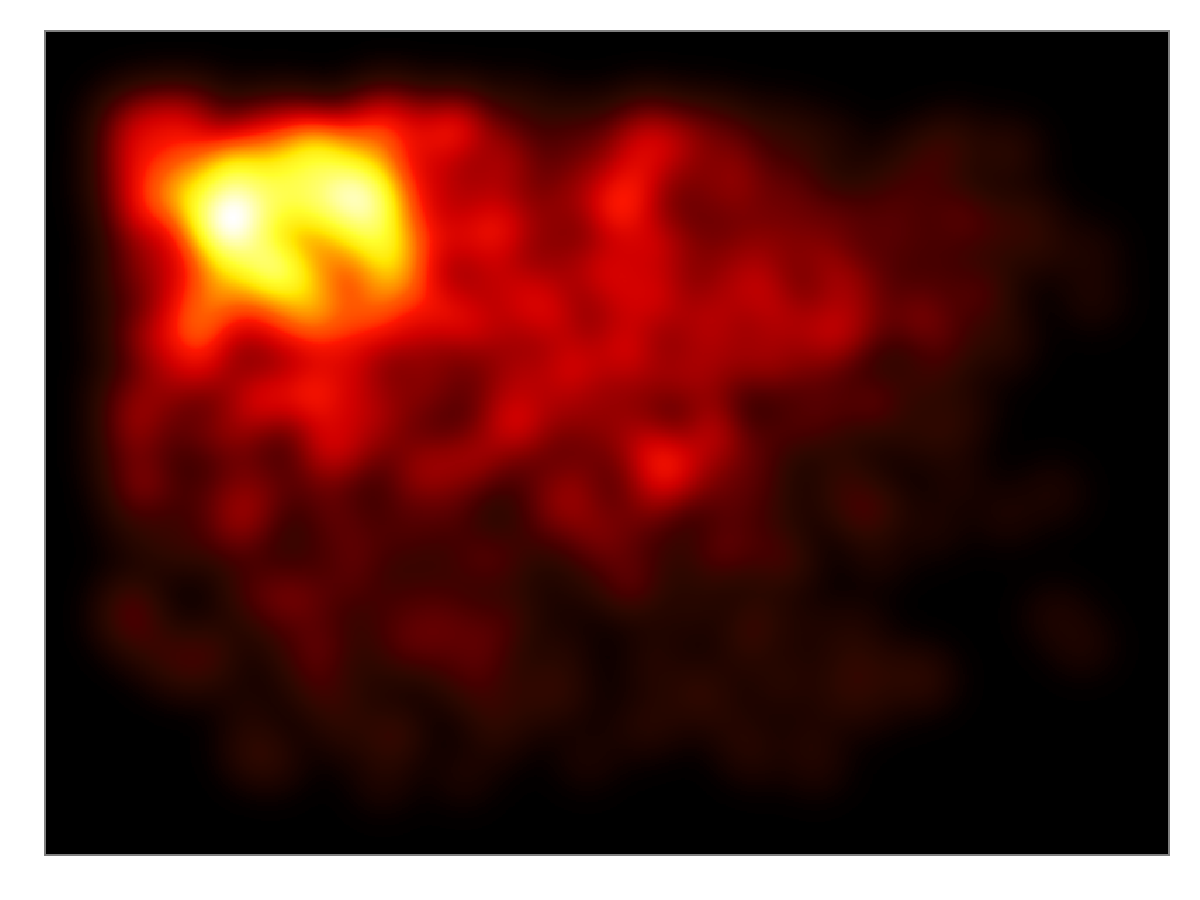
\includegraphics[width=4.5cm]{../scripts/heatmaps/SaccadicFlowMaps/Figures/BBias_11.pdf}}
\subfigure{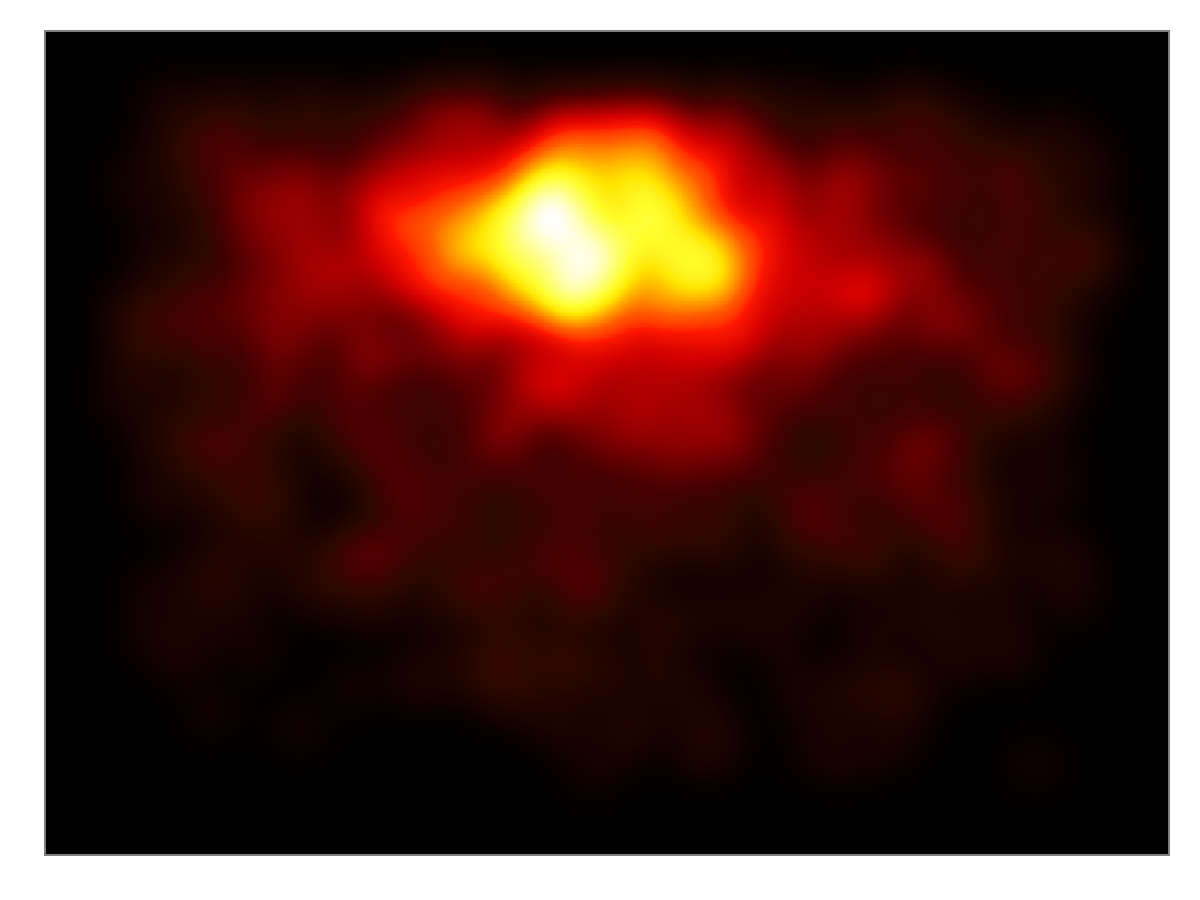
\includegraphics[width=4.5cm]{../scripts/heatmaps/SaccadicFlowMaps/Figures/BBias_12.pdf}}
\subfigure{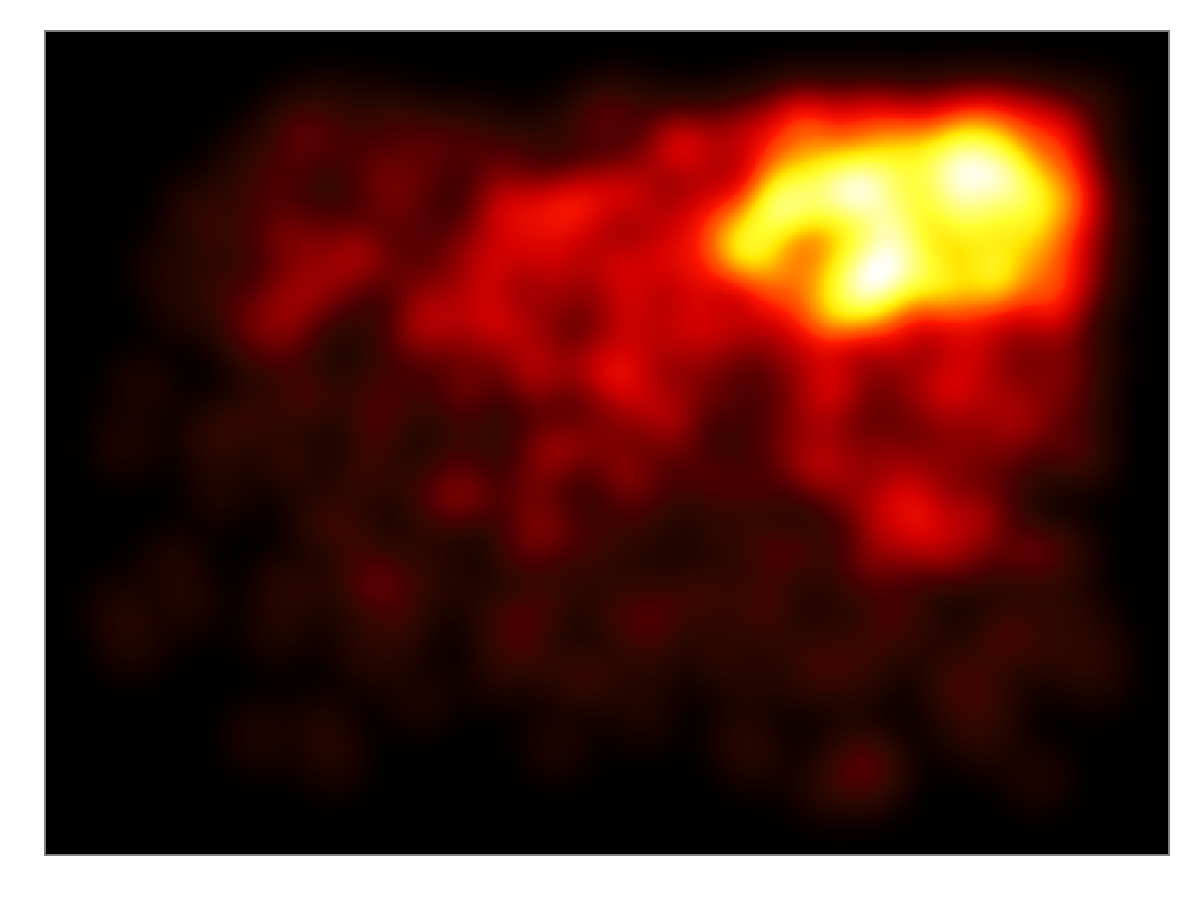
\includegraphics[width=4.5cm]{../scripts/heatmaps/SaccadicFlowMaps/Figures/BBias_13.pdf}}
\subfigure{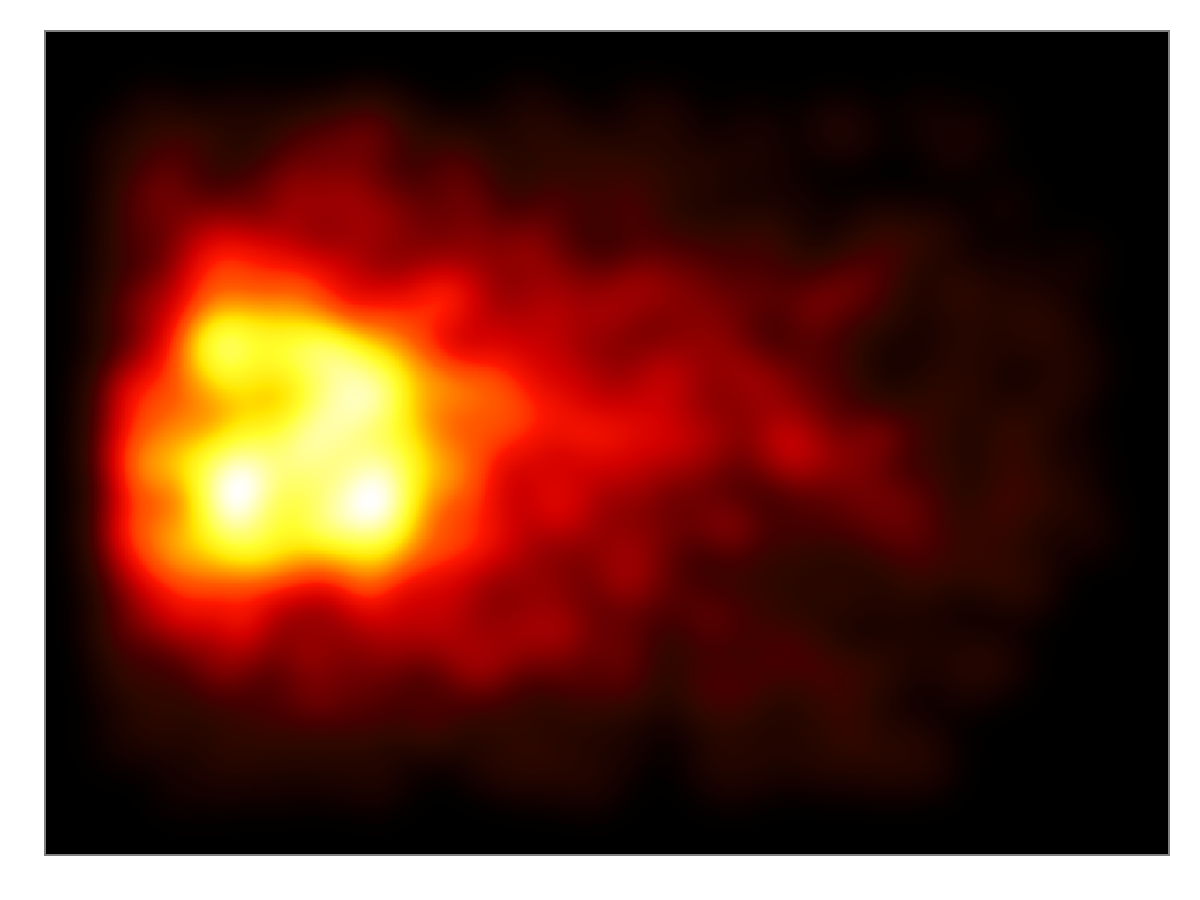
\includegraphics[width=4.5cm]{../scripts/heatmaps/SaccadicFlowMaps/Figures/BBias_21.pdf}}
\subfigure{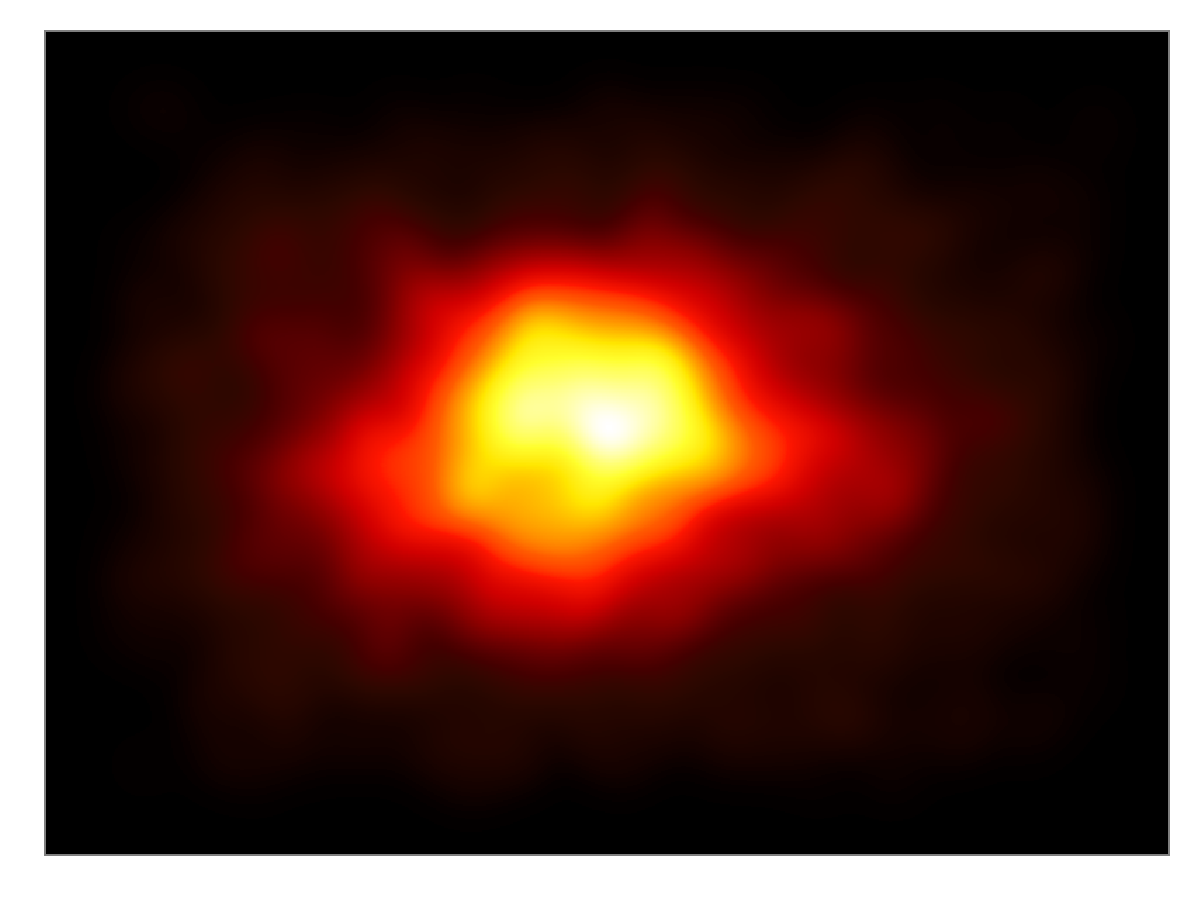
\includegraphics[width=4.5cm]{../scripts/heatmaps/SaccadicFlowMaps/Figures/BBias_22.pdf}}
\subfigure{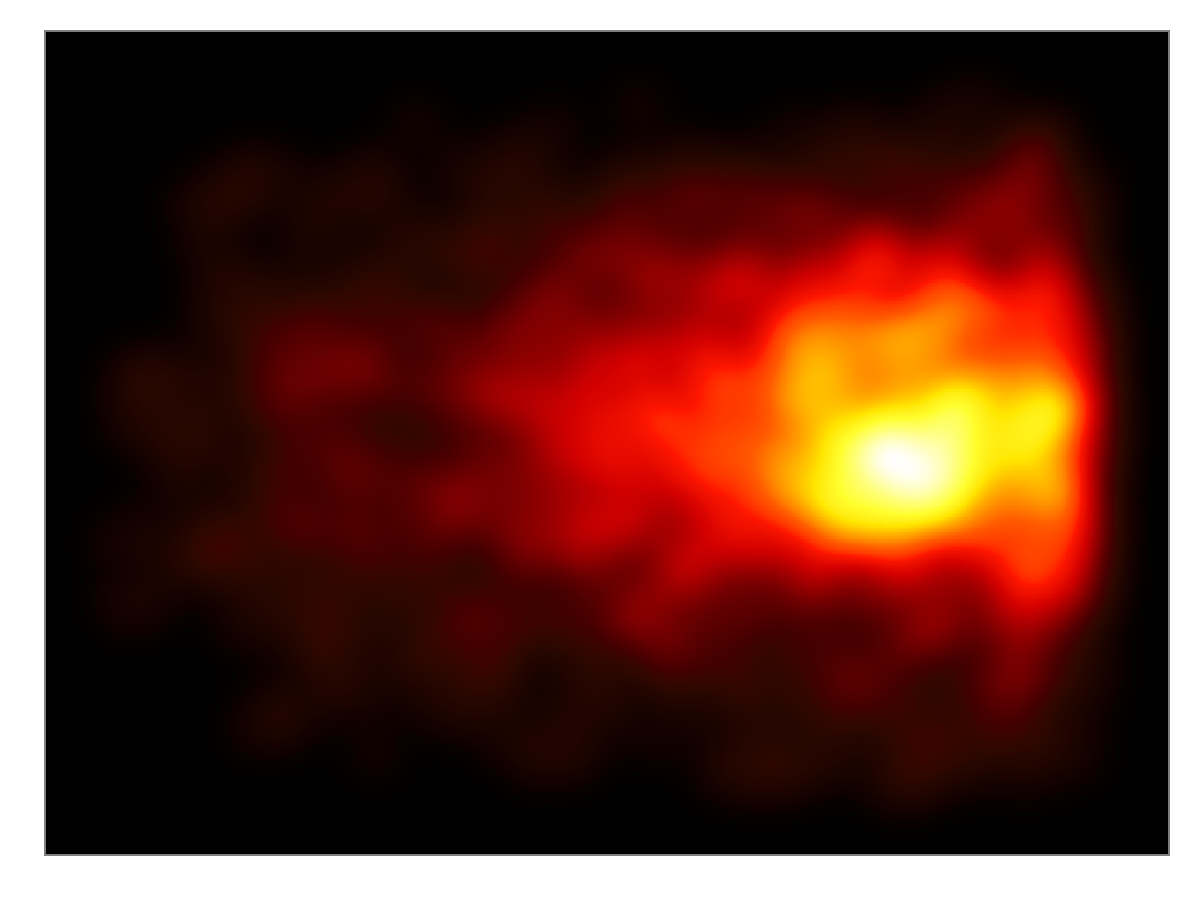
\includegraphics[width=4.5cm]{../scripts/heatmaps/SaccadicFlowMaps/Figures/BBias_23.pdf}}
\subfigure{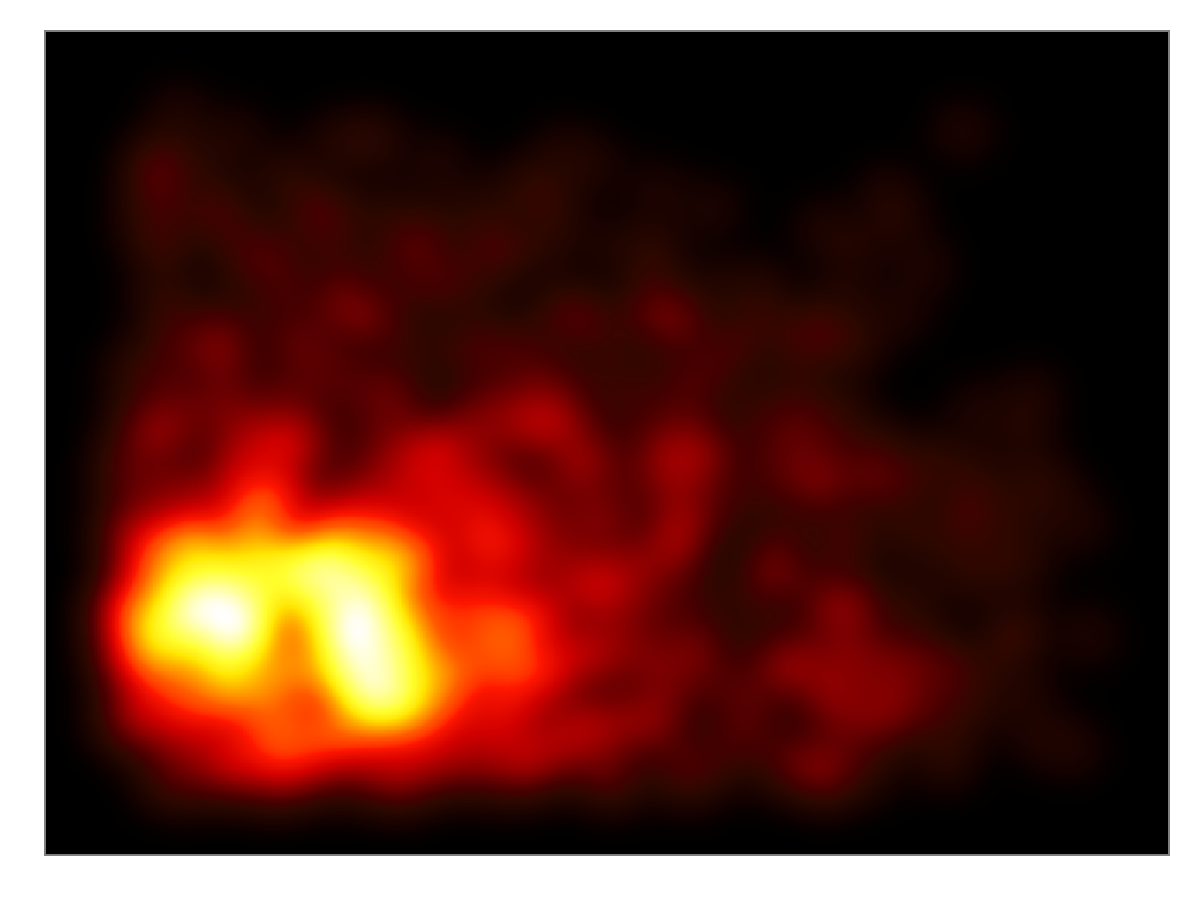
\includegraphics[width=4.5cm]{../scripts/heatmaps/SaccadicFlowMaps/Figures/BBias_31.pdf}}
\subfigure{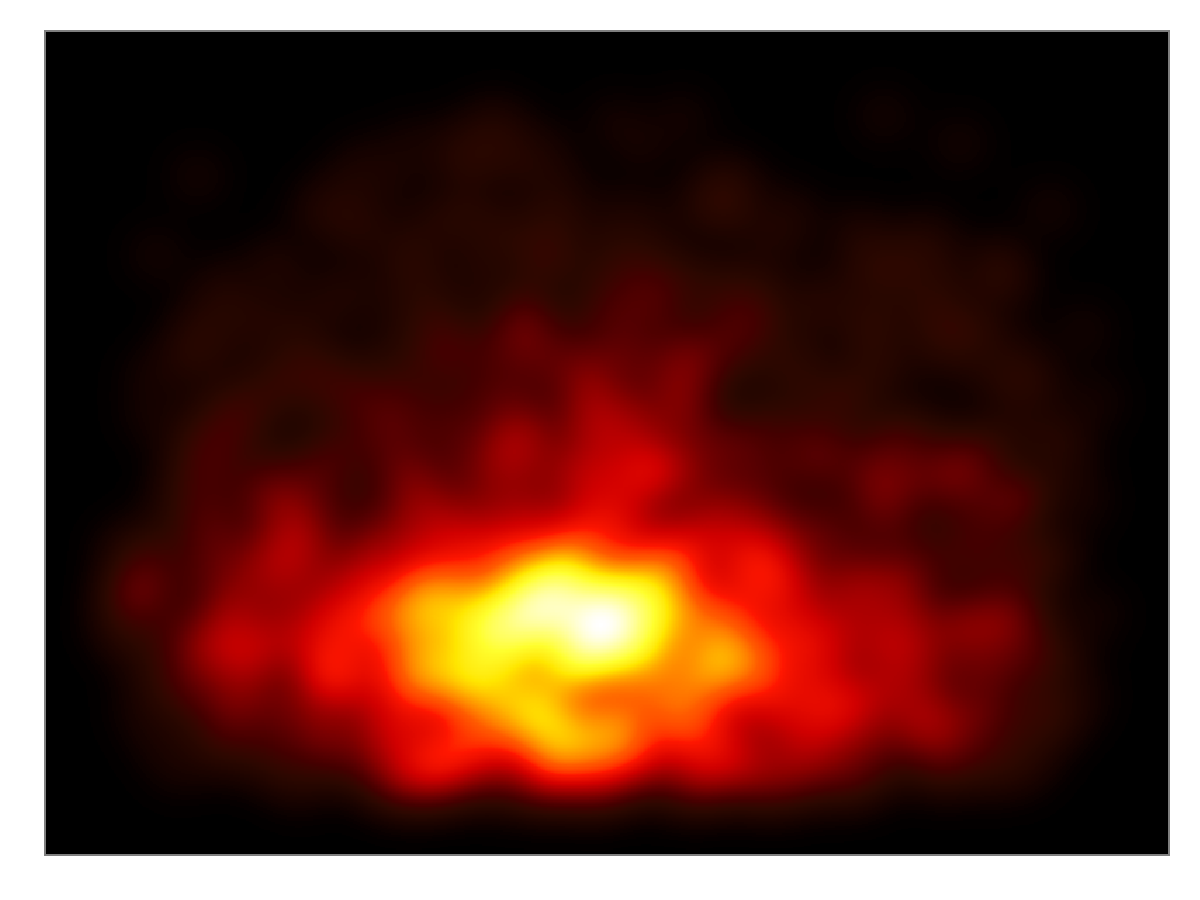
\includegraphics[width=4.5cm]{../scripts/heatmaps/SaccadicFlowMaps/Figures/BBias_32.pdf}}
\subfigure{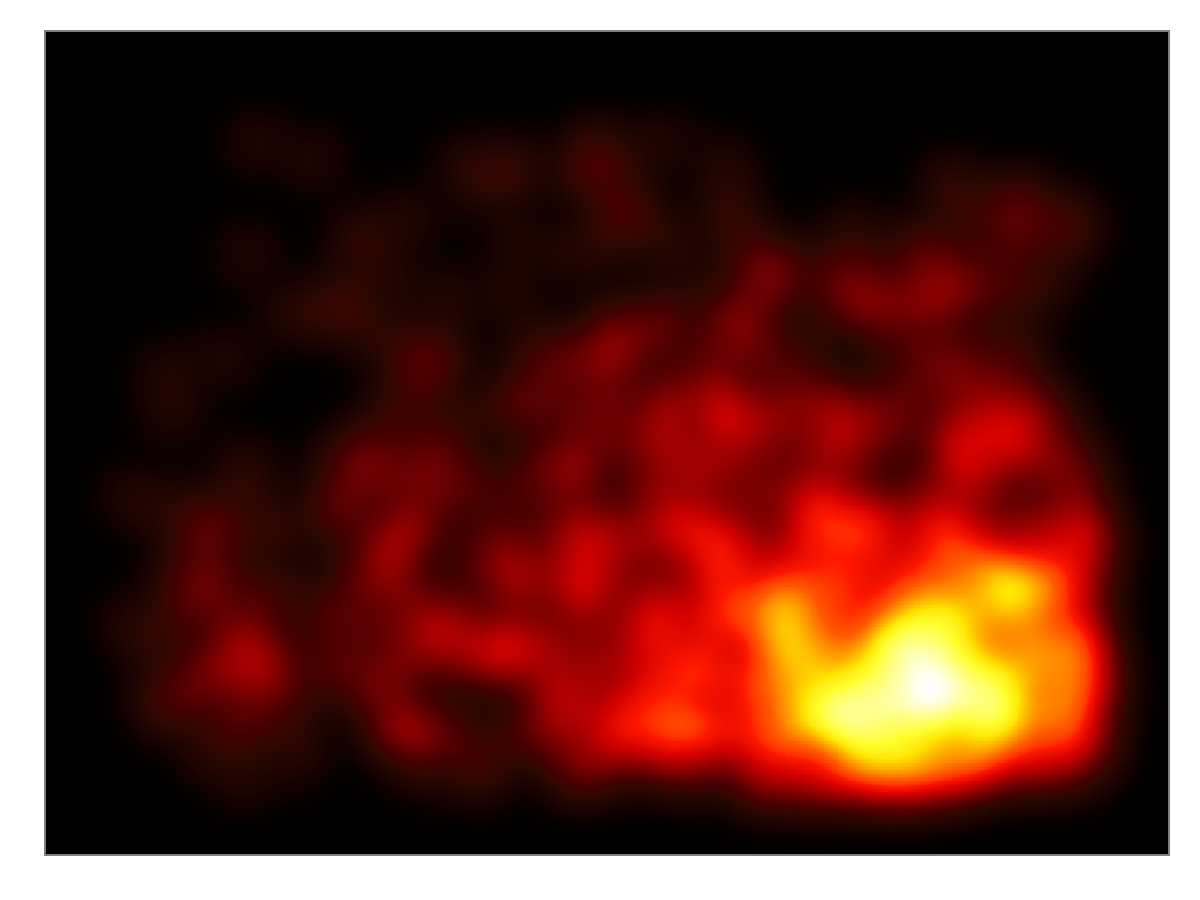
\includegraphics[width=4.5cm]{../scripts/heatmaps/SaccadicFlowMaps/Figures/BBias_33.pdf}}
\caption{Saccade landing positions from fixations that were in different sections of the screen. Data from each plot has been separated into fixations in 9 spatial bins, with the screen being divided into thirds in both horizontal and vertical aspects.}
\label{fig:empiricalSaccadicFlow}
\end{figure*}


\subsection{The central bias}
There is a strong tendency for people to look close to the centre of pictures \citep{Tatler:2007hk,Tatler:2005bw, Canosa:2003tu, clarke_tatler2014} and movies \citep{Tseng:2009jn} presented on computer screens. There have been a number of suggestions for why this might be. One possibility for this effect is that the muscles of the eye show a preference for the `straight ahead' position, re-centring in the orbit of the eye socket for most comfortable contraction of the ocular muscles (an \emph{orbital reserve} \citep{Fuller:1996bx}). As most scene viewing experimental set-ups stabilise the head to increase the accuracy of the eye tracking, and most scenes are presented in the centre of computer displays, such a re-centring mechanism would mean that the centre of images would indeed be preferentially selected. However, when scenes are scrambled into four quadrants, fixations are located near to the centre of each quadrant, rather than the display centre, suggesting that the central tendency is responsive to the viewed content \citep{Stainer:2013ce} rather than the frames of the computer monitor.

Another possibility for the central fixation bias is that it represents a \emph{photographer bias} as photographers tend to frame their shots to include the most important content in the centre of the scene. However, when \cite{Tatler:2007hk} presented scenes where the image features were biased towards the edge of the scene, the central fixation bias persisted. The final possibility is that as a consequence of repeated exposure to photographer bias, the centre of scenes is simply where people are \emph{trained} to look at images \citep{Parkhurst:2002vo}. Such learning of spatial probabilities of targets can explain why, for example, people tend to look around the horizon when searching for people in natural scenes \citep{Birmingham:2009hl, Torralba:2006iq, Ehinger:2009ji}. Expecting to find interesting content in the centre of scenes might be a consequence of this hypothesis typically being correct.

\cite{clarke-tatler2014} revealed that the characteristics of the central bias is remarkably consistent across a series of eye movement databases.... Mention \cite{nuthmann2015} who recently ran this bias on a new dataset and confirmed it accounted for more of the data than an isotropic Gaussian.

\subsection{Behavioural biases in saccades}
Further to the observed bias towards the centre of images, it has been revealed that there are underlying biases in the characteristics of eye movement (in terms of the directions and amplitudes of saccades). It has been noted by several researchers that when viewing scenes, there is a higher proportion of eye movements in horizontal directions than vertical or oblique movements (Brandt, 1945; Crundall \& Underwood, 1998; Gilchrist \& Harvey, 2006; Foulsham, Kingstone \& Underwood, 2008; Tatler \& Vincent, 2008). There are a number of possibilities as to why this tendency exists (as discussed in Foulsham, Kingstone, \& Underwood, 2008). Firstly, there may be a muscular or neural dominance making oculomotor movements in the horizontal directions more likely. Secondly, the characteristics of photographic images may mean that content tends to be arranged horizontally by the photographer. In such situations, horizontal saccades may be the most efficient way to inspect scenes. Thirdly, using horizontal saccades in scene viewing might be a learned strategy. Observers may learn the natural characteristics of scenes based on previous experience, and therefore demonstrate an increased likelihood of moving in the horizontal direction. A final alternative explanation is that this tendency is a consequence of the aspect ratio of visual displays, which normally allow for larger amplitude saccades in the horizontal than vertical directions (Wartburg et al., 2007).

Foulsham and colleagues have presented two interesting exceptions to the horizontal direction bias. Foulsham, Kingstone and Underwood (2008) found that when the orientation of an image is rotated, the distribution of saccade directions follows the orientation of the scene. A second exception comes from using circular apertures \citep{Foulsham-kingstone2010}. When a scene is presented in a circular aperture, the tendency to make horizontal saccades disappears, being replaced by a tendency to make vertical saccades relative to the image orientation. However, when using fractal images (where images do not have an obvious orientation), observers tend make horizontal saccades, regardless of the angle that the image is presented.

\subsection{The present study}
The aim of the present study is to characterise the underlying biases of eye movement with which to understand fixation selection in natural scenes. We extend the previous work by examining [XXstuffXX] and 


%%%%%%%%%%%%%%%%%%%%%%%%%%%%%%%%%%%%%%%%%%%%%%%%%%%%%%%%%%
\section{Using Biases}
\label{sec:usingbiases}
%%%%%%%%%%%%%%%%%%%%%%%%%%%%%%%%%%%%%%%%%%%%%%%%%%%%%%%%%%

This section makes use of an improved central bias model and the \textit{saccadic flow} model (described in Section \ref{ModellingFlow}). The new central bias model is similar to the model presented by \cite{clarke-tatler2014}, except for using a truncated Gaussian distribution to take the image boundaries into account. We present three examples of how these bias models can be used as priors in order to weight fixations, based on the fact that Flow produces likelihoods for any given fixation given the current fixation. First of all, we will demonstrate how we can weight fixations in gaze landscapes (also known as hotspot maps or heatmaps) to reduce noise and to give an improved visualisation of the image regions participants looked at more than expected. Secondly, we examine whether saccadic flow can be used to better understand the contribution of low-level features on fixation selection, and potentially lead to better evaluation of such computational saliency models. Finally, we demonstrate how flow can be used to generate a series of saccades, and compare these to observed human saccades. Being able to generate realistic synthetic datasets is useful to create an image-independent baseline with which to examine spatial maps of prediction using signal detection theory \citep[see][]{clarke-tatler2014}.

\subsection{Gaze landscapes}

One technique that is commonly used to visualise the spatial allocation of gaze is to create 'heatmap' plots where colour or luminance is used to indicate the density of fixation on those locations (Figure ~\ref{fig:adjustedHeatmaps}, column 2). A potential problem with visualising data in this way is that such maps represent all fixations as being of equal importance. For example, a location that is fixated for one second would be weighted equally with fixations that lasted half that time. If we want to make an assumption that fixation duration is intimately linked with the importance of that fixation (i.e. we will look longer at more informative information) then we can change our visualisation to weight fixations by their duration (Figure ~\ref{fig:adjustedHeatmaps}, column 3). \textbf{However, this weighted heatmap still fails to distinguish fixation behaviour likely to arise from image independent biases like the central fixation bias from fixation behaviour likely to reflect meaningful interrogation of, and response to, the viewed content.} 

\begin{figure*}
\centering
\includegraphics[width=13cm]{figs/heatmap_figure.pdf}
\caption{Examples of fixation heatmap plots from \cite{clarke2013}. The same fixations are presented where the Gaussian at each fixation is weighted by the duration of the fixation, the centre bias model from \cite{clarke-tatler2014} , and the saccadic flow model presented in this paper.}
\label{fig:adjustedHeatmaps}
\end{figure*}

An advantage of the \citet{clarke-tatler2014} model and the saccadic flow model presented here, is that we can represent fixations by the likelihood that they would occur based on the predictions of the models. Because the models reflect image-independent behavioural and oculomotor biases, fixations not predicted by these models might involve more high-level mechanisms. For example, given a tendency to fixate in the centre of the scene, we might consider saccades to non-central locations to be less predicted and therefore more likely to be image- or task-related.  In Figure ~\ref{fig:adjustedHeatmaps} (column 4 and 5) we present some overlaid heatmap data from the \citet{clarke2013} dataset, where fixations are weighted by the inverse probability of them occurring based on the models of central bias and saccadic flow. These figures reveal that representing data in this manner can allow us to visualise information that was important enough to disrupt these biases. In other words, these visualisations  remove some of the image-independent biases, and reveal the more important image \emph{dependent} information.


The top row of Figure ~\ref{fig:adjustedHeatmaps} demonstrates that weighting the fixations by the central bias and flow model both reduce the \emph{importance} of some fixations. The central bias model punishes fixations near the center of the image, while the flow model punishes fixations that were well predicted by the oculomotor biases of the saccadic flow model. Conversely, the models reward unlikely fixations. The second row reveals an instance of where the car to the left received less fixations than the pub sign, but that these fixations are boosted in the central bias and saccadic flow models where 'unlikely' saccades were made to this location. In the third and fourth rows, there are examples of images with important content near the centre of the photograph. This illustrates how the central bias model can sometimes over-compensate and reduce the influence of fixations in the centre of pictures that have important content located there. Given the tendency for photographers to centre their photographs around important content, reducing the weight of fixations to the castle in the painting (row 3) and the girl's face (row 4) would perhaps overly punish centrally biased photographic composition. With the flow model, however, these areas are still represented, as observers made saccades to theses regions that were unlikely to be driven by behavioural biases.

\subsection{Removing biases when examining image-dependent information}

By considering saccades in light of the probability that they were generated by image-independent biases, we can gain further insights into the image-dependent features that are important in attracting fixation. One feature that has been shown to correlate with fixation is visual salience \citep{parkhurst2002}. However, others have argued that this tendency is driven by the correlation between salient objects and their semantic interest \citep{henderson2007}, with interesting objects tending to be placed near to the centre of photographs \citep{tatler2007}. Oculomotor biases which favour a central tendency would predict the same fixation placement regardless of the distribution of salient objects in the image \citep{tatler-vincent2009}. Here, we can examine this question by looking at the relationship between saccade probability and the ability of different conspicuity maps to predict fixation. We can therefore examine how the effect of visual salience observed in eye movement analysis is related to the behavioural biases of eye movements.

We compared the proportion of fixations that fell in the brightest 20\% of pixels for salience maps to the likelihood of fixations from the flow and central bias models. Fixations were separated for each image into bins of 5\% from the least-likely to the most-likely to be generated based on salience. We then examined what proportion of each of these bins were in the brightest 20\% of salience maps using the Adaptive Whitening Saliency (AWS; \cite{garciadiaz2012}), RARE \citep{riche2013} and Graph-based visual saliency \citep[GBVS;][]{harel2006} algorithms. We selected AWS and RARE as they are the two best performing salience models according to the MIT Saliency Benchmark \citep{mit-saliency-benchmark,judd2012} with publicly available code, and GBVS as it contains a bias towards the centre cause by summing neighbouring pixel values across the spatial prediction map.

Figure ~\ref{fig:salmaps} reveals that the likelihood of making a saccade based on both the central bias and the flow model is highly related to salience in both AWS and RARE, with low-likelihood saccades being less likely to be to a salient region. Saccades that are very unlikely to be generated based on the oculomotor tendencies of eye movement (both flow and central bias) are therefore also less well explained by salience. Of the 5\% of fixations that were \textit{most} likely from saccadic flow, ~60\% of fixations fell in the 20\% thresholded region of the AWS map. However, of the 5\% of fixations that were \textit{least} likely from saccadic flow, only 40\% of fixations fell in this region. This means that it may be important to consider, and potentially remove, behavioural biases when attempting to predict fixation selection using feature-based models to ensure that any benefit in predictive power cannot be explained by behavioural biases correlating with salience. When examining a model that contains an inherent central bias (GBVS), we can see that weighting fixations by the \citet{clarke-tatler2014} central bias model is highly related to the performance of GBVS in predicting fixation selection.

%Examples of the maps can be seen in Figure \ref{fig:salmaps}. Salience maps were normalised to sum to 1, and data were analysed using linear mixed-effect models with the fixation weighting (duration, central bias or saccadic flow) as fixed effect factors, and image and participant as random effects. 

\begin{figure}
\centering
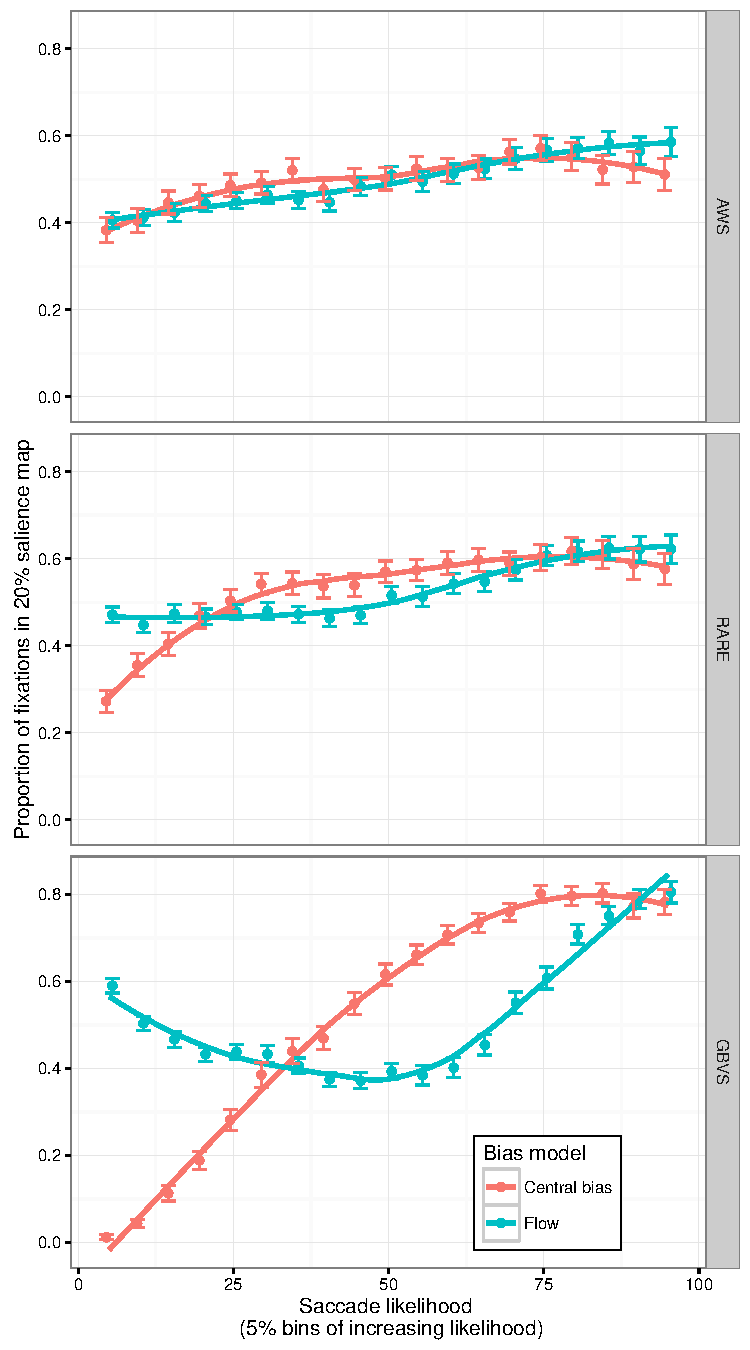
\includegraphics[width=\columnwidth]{figs/SaccadeSaliency.pdf}
\caption{Saccades binned by probability of them occurring in 5\% bins against the proportion of those fixations that fell in a 20\% thresholded region of AWS, RARE and GBVS salience maps.}
\label{fig:salmaps}
\end{figure}



\subsection{Saccadic Flow as a Generative Model}
\label{sec:humanComp}

Another use of the saccadic flow model is that it allows us to make spatial maps that relate to the probability of \emph{all saccades within a scene} based on the current position. For example, Figure~\ref{fig:flowPredict} shows that for three fixations in different locations within a scene, flow will make different spatial predictions of the next saccadic landing position. We can use this method to generate sequences of synthetic scan-paths. Here, we compare the distributions of these generated scan-paths with empirical scan-paths to determine which aspects of human saccadic behaviour are not captured by our model. To do this, we will create a merged dataset of fixations from the eight training datasets (175 000 fixations, including initial fixations, in total over 16 000 trials), and then generate a matched synthetic dataset such that the number of fixations in each trial is identical. 

\begin{figure*}[htb]
\centering
\subfigure[]{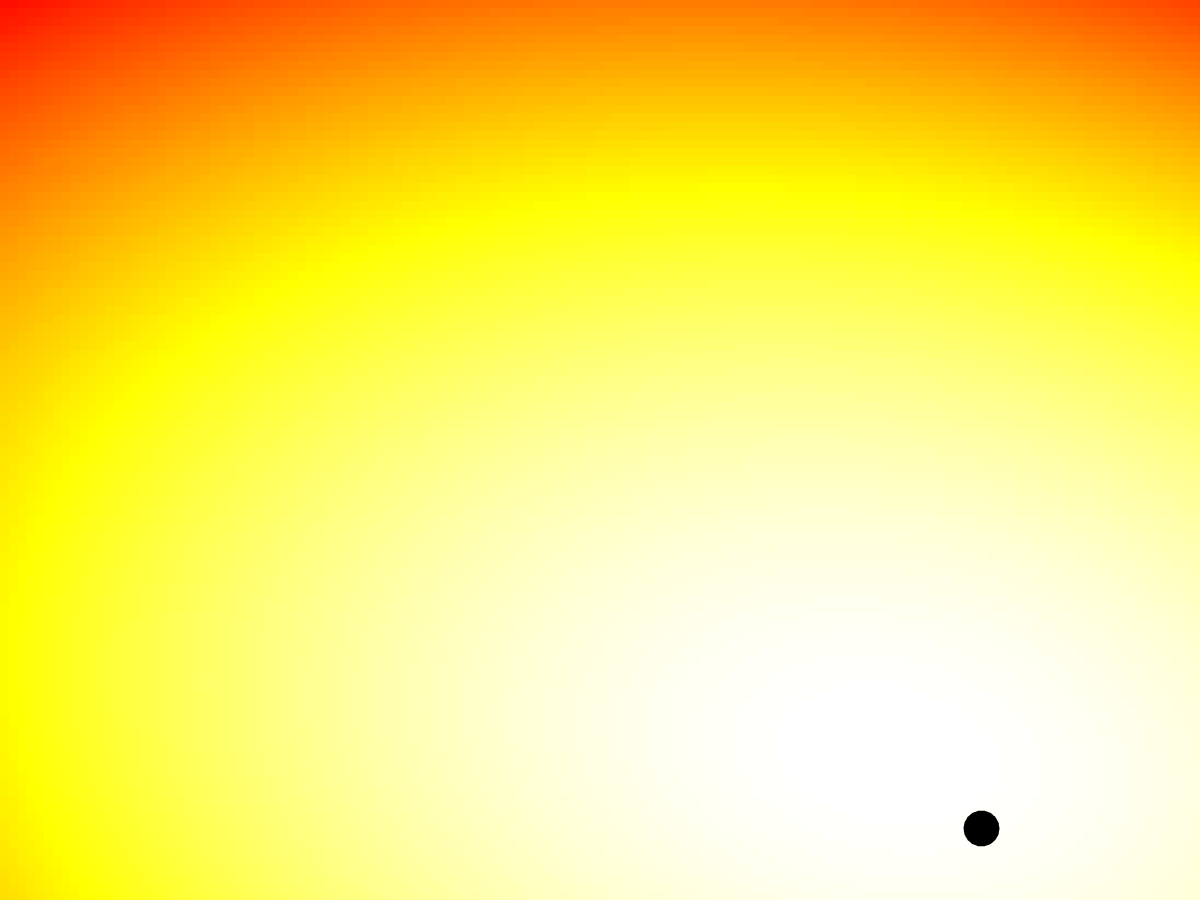
\includegraphics[width=4.2cm]{figs/DownLeft.png}}
\subfigure[]{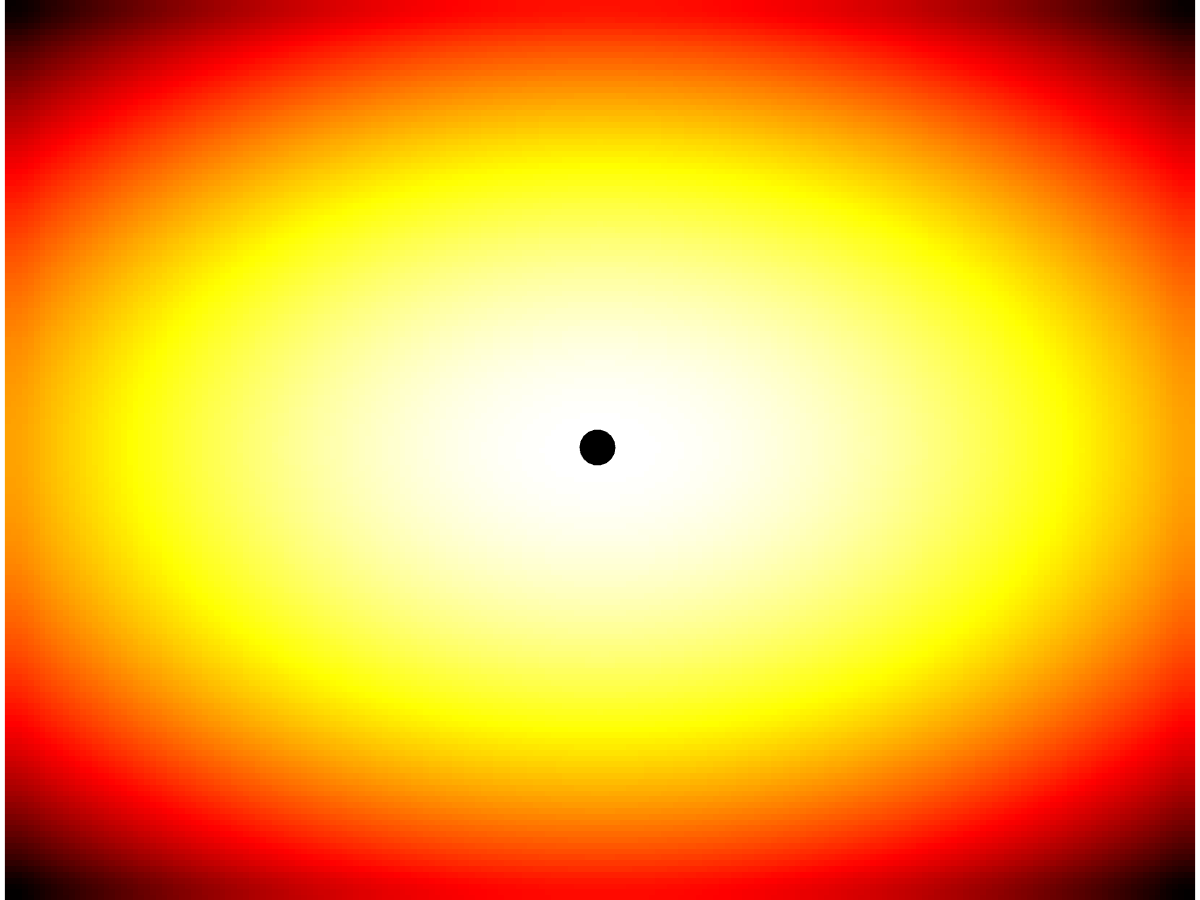
\includegraphics[width=4.2cm]{figs/Center.png}}
\subfigure[]{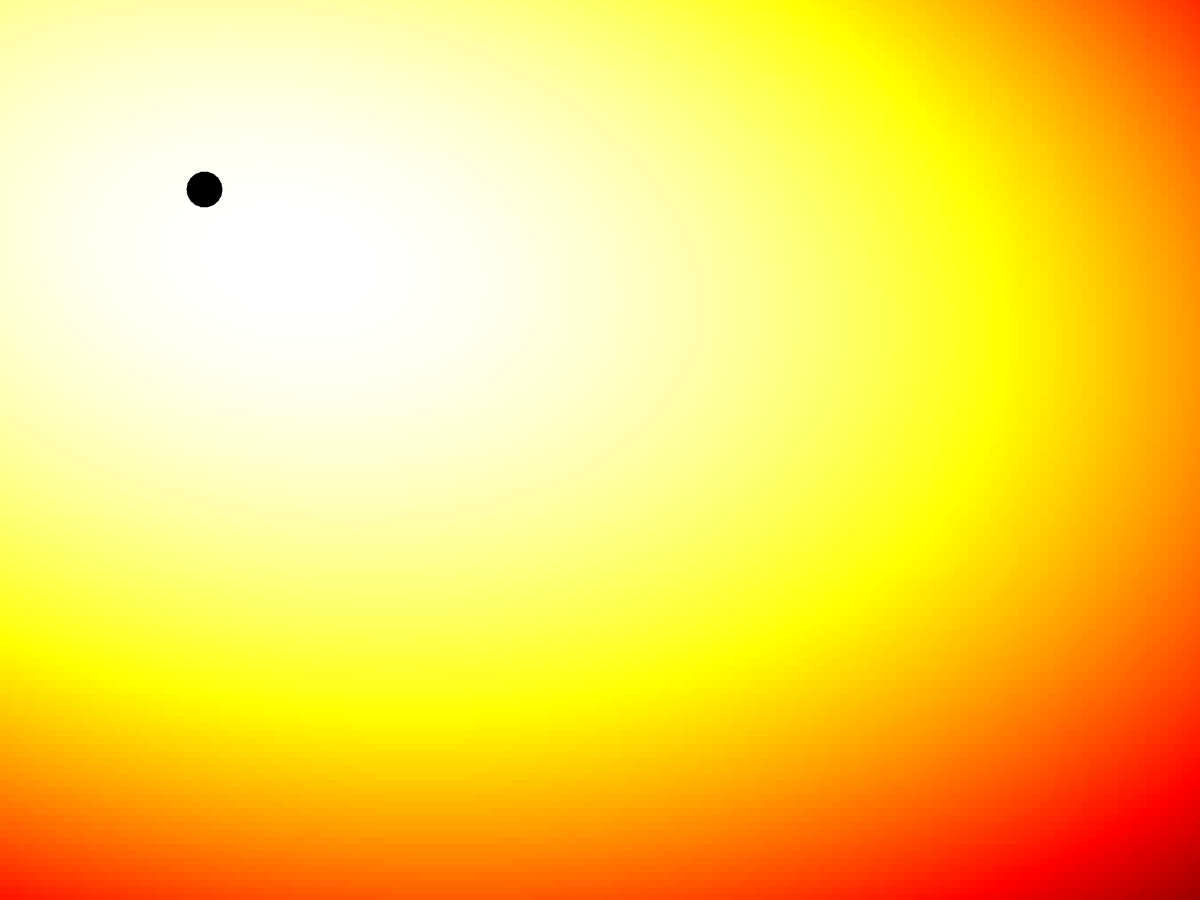
\includegraphics[width=4.2cm]{figs/UpRight.png}}
\caption[]{Example spatial prediction maps for all potential saccade locations from 3 different fixation positions (black circles), to demonstrate how flow's predictions differ across the extent of a scene.}
\label{fig:flowPredict}
\end{figure*}

We can see from Figure \ref{fig:flowHumanComp}(a) and (b) that both the central bias and the saccadic flow model do a good job of capturing the distribution of fixation locations over the $x$ and $y$ axes. While it is not surprising that the central bias closely matches the empirical distributions (as this is exactly what it has been fitted to), it is interesting that saccadic flow does just as good a job. Hence, the central bias can be thought of as a property of saccadic flow, and does not need to be accounted for separately. 

When compared to the empirical distributions, both the central bias and saccadic flow appear to be slightly biased towards making fixations to the extreme edges of the image. This suggests that the truncated Gaussian distribution does not quite capture the effects of the image boundary on fixation selection and there is some additional aversion to fixating close to the screen edge. 

Another discrepancy between the synthetic and empirical distributions can be seen with saccadic amplitudes. While the flow model is a better fit to the human data than the central bias, it still underestimates the proportion of very short saccades (Figure \ref{fig:flowHumanComp}(c)). Interestingly, the flow model does manage to capture the initial increase in saccadic amplitudes after scene onset (Figure \ref{fig:flowHumanComp}(d)), but it does not explain the subsequent coarse-to-fine dynamics that are seen in the empirical scan-paths. 


\begin{figure}[htb]
\centering
\subfigure[]{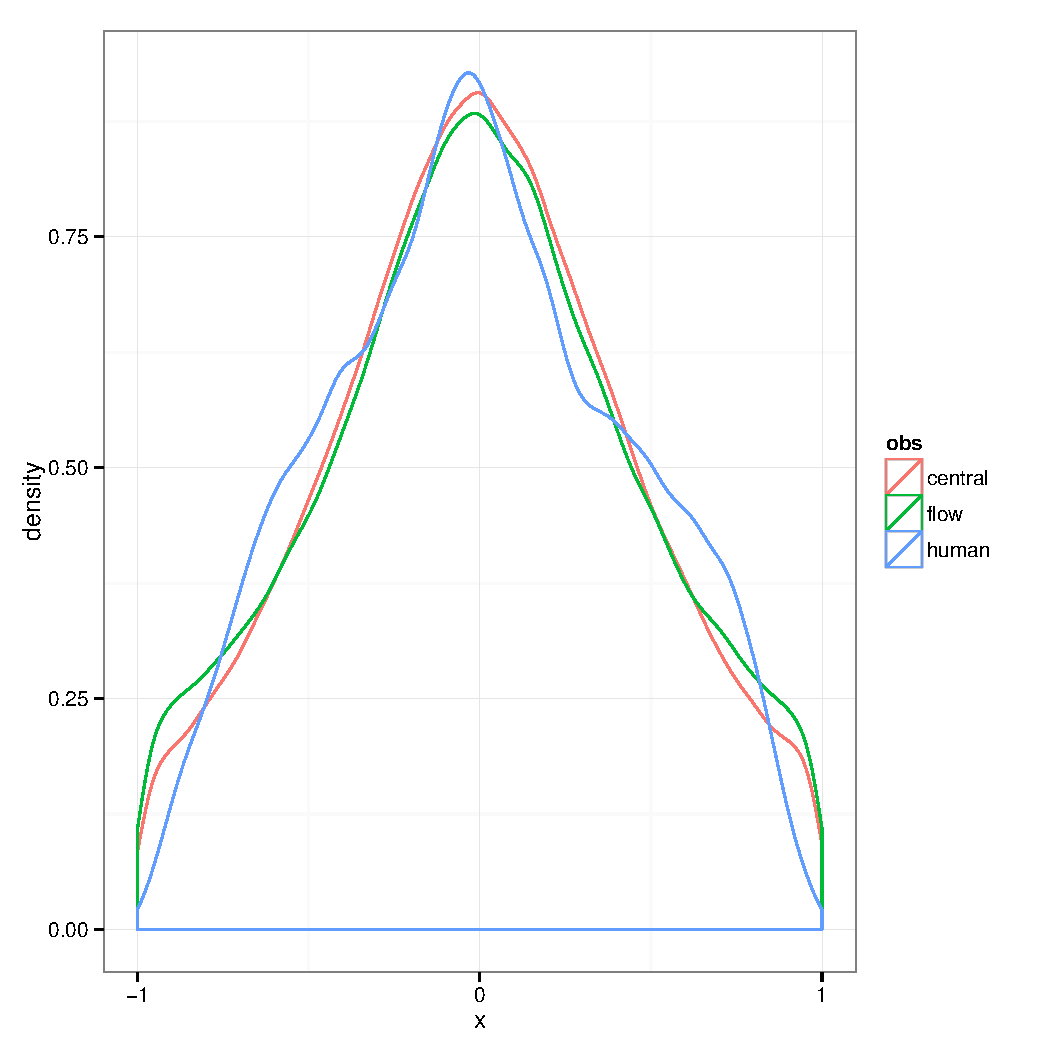
\includegraphics[width=3.8cm]{../scripts/coarse2fine/figs/xFixComparison}}
\subfigure[]{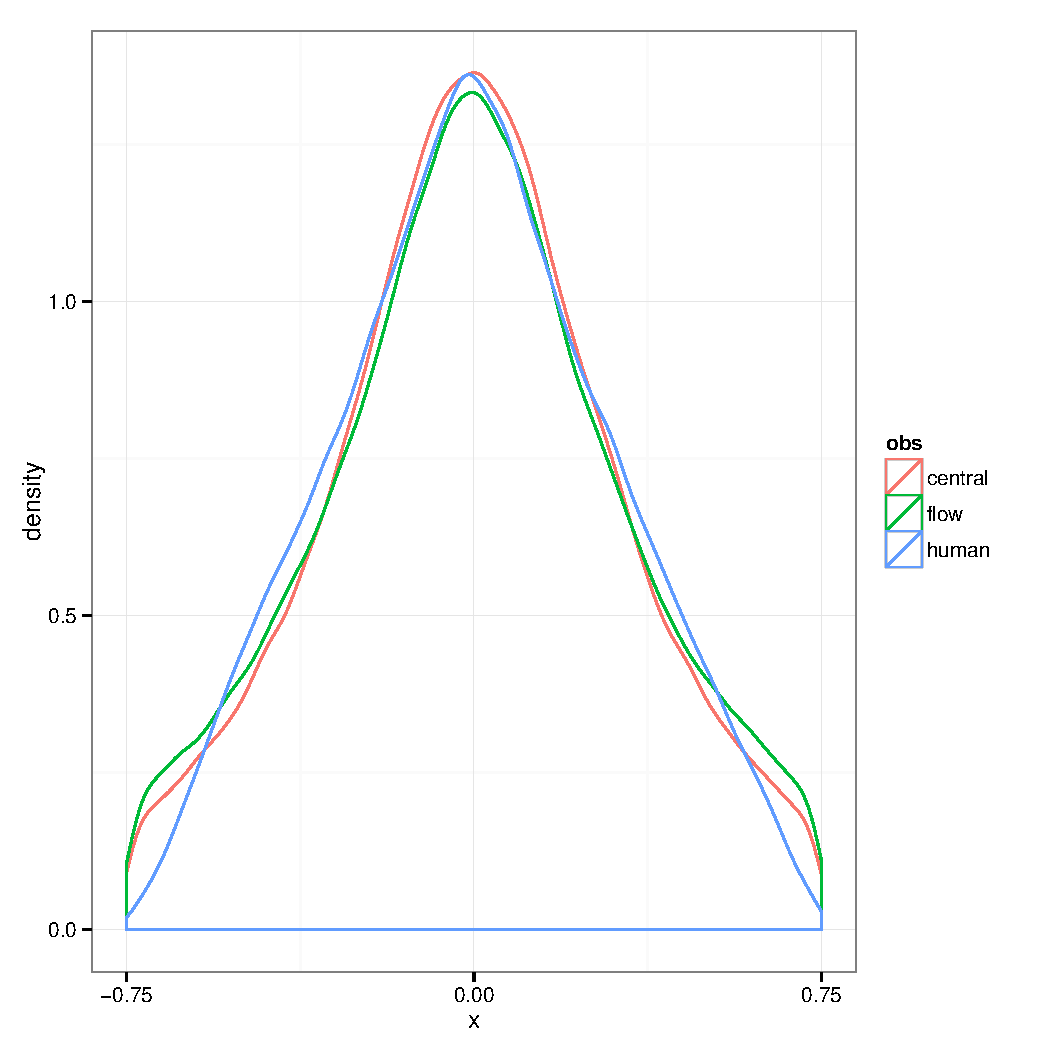
\includegraphics[width=3.8cm]{../scripts/coarse2fine/figs/yFixComparison}}
\subfigure[]{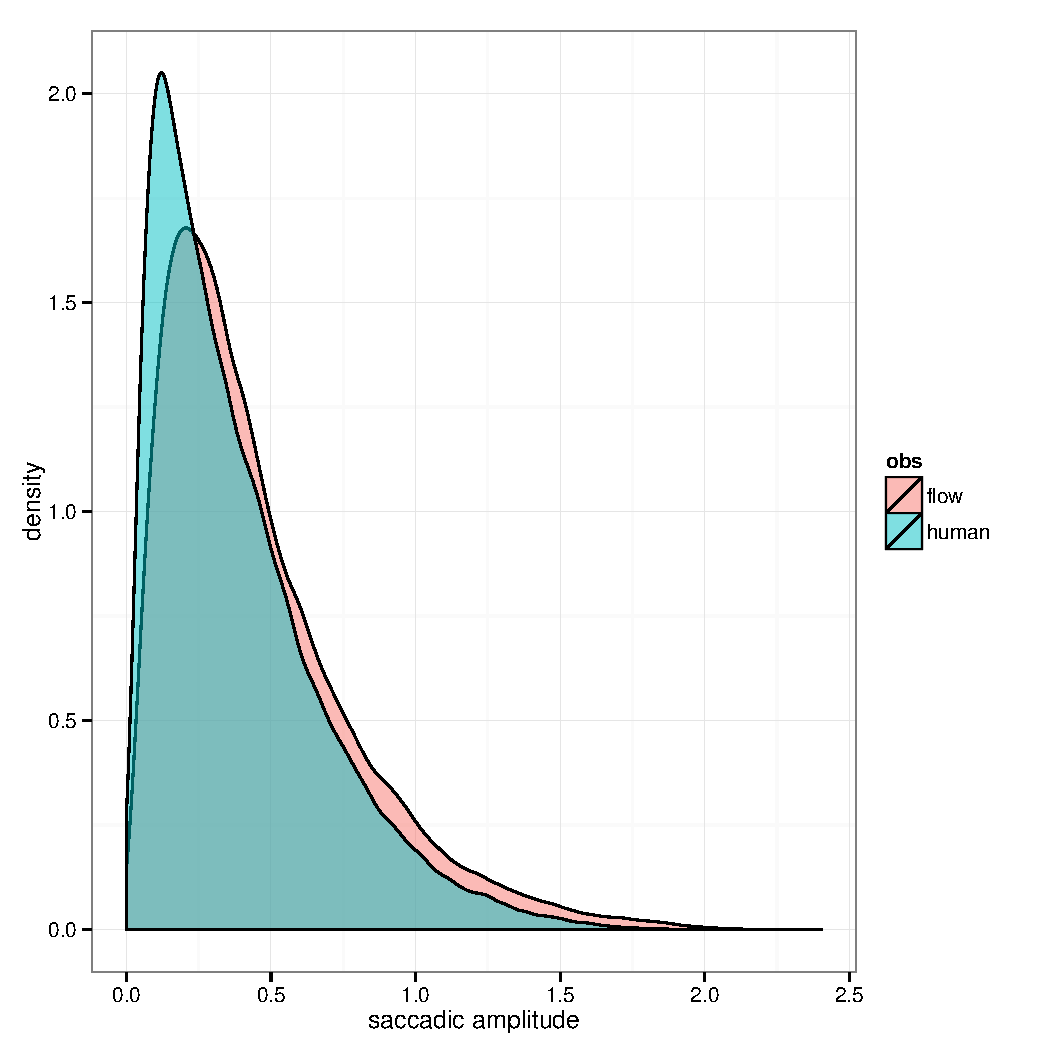
\includegraphics[width=3.8cm]{../scripts/coarse2fine/figs/ampSaccComparison}}
\subfigure[]{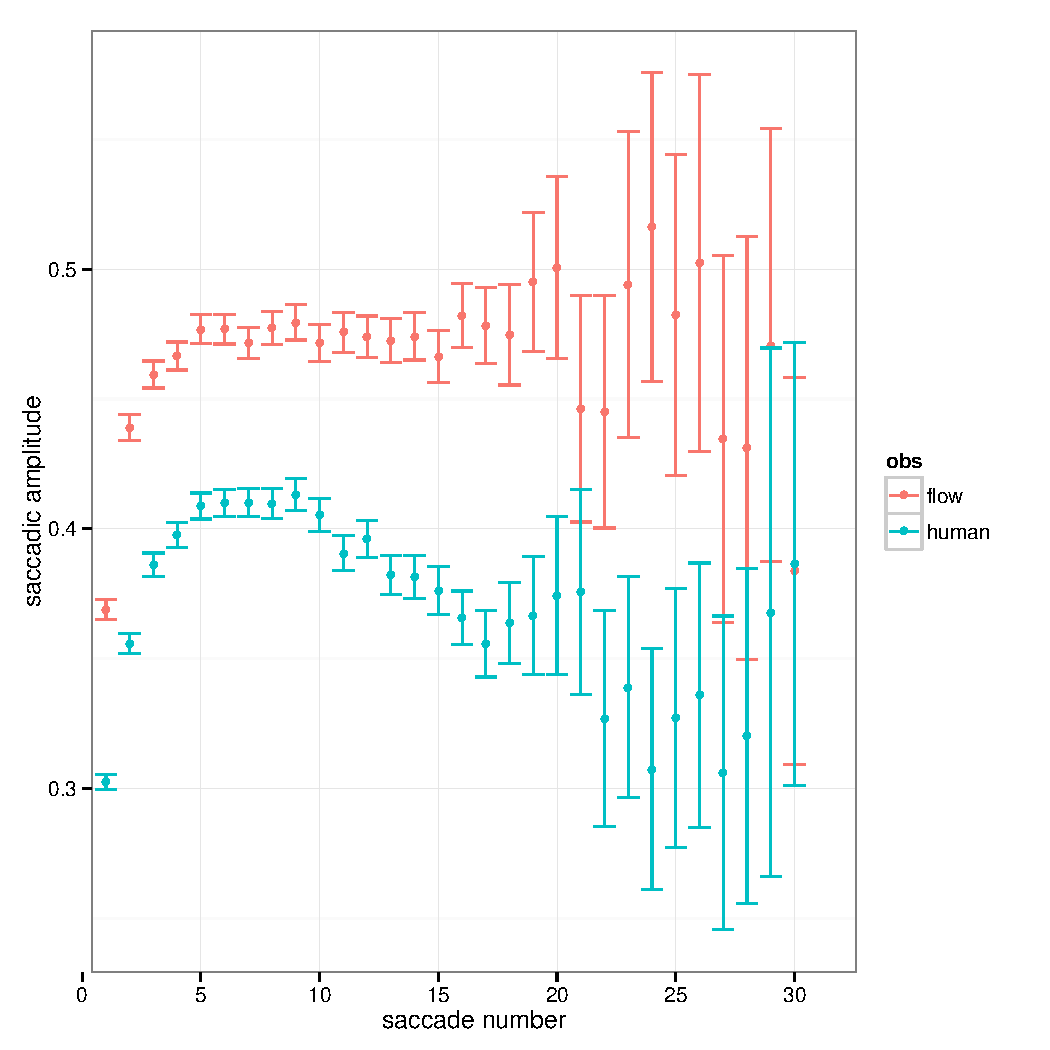
\includegraphics[width=3.8cm]{../scripts/coarse2fine/figs/saccAmpOverTimeFlow}}
\caption[]{\textit{blue}: human, \textit{red}: central bias, \textit{green}: saccadic flow. \textit{top row}: Comparison of $x$ and $y$ fixation positions between human fixations and synthetic points generated from the central bias and flow model. \textit{bottom row}: We can see that the flow model consistently makes saccades with a slightly larger amplitude than human observers. Distances are expressed relative to the width of the image. Best fit line in (d) fitted with loess regression. All distances are given in normalised units in which the width of an image is 2 (see Section \ref{sec:modellingMethods}).}
\label{fig:flowHumanComp}
\end{figure}


\subsection{Saccadic Flow across different tasks}


\subsection{Discussion}

We have demonstrated different ways biases such as saccadic flow and the central bias can be used in eye movement research. They can be used as a prior on the probability of making saccades to different regions of the image, allowing us to then more clearly visualise the image-dependant behaviour. We have also shown that the likelihoods of fixations under the bias models are related to features such as salience. The interpretation of visual salience as a predictive model of fixation selection can therefore be informed by considering how likely a saccade is to be generated by these models. Finally, we can also use the bias distributions to generate synthetic data that can be used as control points in ROC analysis, and to explore which aspects of human saccadic dynamics are not captured by the simple flow model. 
>>>>>>> Flow-2.0



\section{Modelling Biases}
\label{sec:biases}

In this section, we will present an updated central bias distribution (using a truncated Gaussian); explore the degree of asymmetry in viewing positions, and describe the saccadic flow model. 


%%%%%%%%%%%%%%%%%%%%%%%%%%%%%%%%%%%%%%%%%%%%%%%%%%%%%%%%%%
\subsection{Modelling Methods}
%%%%%%%%%%%%%%%%%%%%%%%%%%%%%%%%%%%%%%%%%%%%%%%%%%%%%%%%%%

In this section, we will give an overview of the methods and data used for the saccadic flow modelling.

\subsubsection{Datasets}

We will uses a number of previously published datasets. The models will be trained on a subset of the 10 datasets used in \cite{clarke-tatler2014}. These data are taken from \cite{clarke2013, tatler2005, tatler2007, yun2013, einhauser2008,judd2009}. The inital saccade after image onset ($9.1\%$ of the data) are excluded, giving us a total of 159,226 saccades. We chose to remove the data from \cite{asher2013} from our training set as the images have an aspect ratio of 5:4, whereas the rest of the data in our training set has an aspect ratio of 4:3. The pedestrian search dataset \citep{ehinger2009} was removed from the training set as previous analysis \citep{clarke-tatler2014} shows that it appears to be biased compared to the other datasets. Both these datasets are now used as test sets to evaluate how well our models generalise. 

We also add a number of other datasets to our test suite collection. 
\begin{itemize}

\item \cite{jiang2014} collected data from 16 observers viewing 500 natural scenes containing crowds of people (aspect ratio 4:3).

\item \cite{clarke2009} has a dataset of fixations made during a visual search for a target on a homogeneous textured background (i.e. target in noise). This dataset differs from the previous in that there is no semantic image content in the scene, and the stimuli had a 1:1 aspect ratio.

\item \cite{greene-wolfe2012} released a dataset of observers viewing square greyscale photographs.

\item \cite{borji2015} recently released a very large ($\approx 0.625$million fixations, 2000 images) dataset collected over twenty different stimuli types. Given the size of this dataset, and the widescreen 16:9 aspect ratio, the evaluations on this dataset are presented seperately, and split by stimuli class.

\end{itemize}

An overview of the datasets used is given in Appendix Tables \ref{tab:datasets} and \ref{tab:setuptable}.

\subsubsection{Pre-processing}

As with \cite{clarke-tatler2014} we have normalised all fixations to the image frame, keeping the aspect ratio constant. ie, $(x,y)\in (-1.-1)\times(-a,a)$ with typically $a=0.75$. The initial fixations and saccades were not included in the analysis. Saccades with a start or end point falling outside of the image frame were also removed. 

When fitting saccadic flow models,  we \textit{mirrored} the set of fixations, but adding in reflected copies of the data (reflected in the horizontal, vertical and both midlines). This has two advantages. (i) It is an easy way to make saccadic flow biases in the horizontal or vertical directions. This is similar to how the central bias was defined \cite{clarke-tatler2014}, but by a different mechanism (with the central bias, the model fitting procedure is much simpler and so we just enforced zero mean and 0s in the covariance matrix). (ii) It increases the amount of data available for fitting by a factor of four. This is important as (due to the central bias) there are relatively few saccades that originate from the corners of the images. By equating all corners, we can pool the data and obtain more stable estimates for the underlying distribution. 


The downside of mirroring saccades in this manner is that our model of saccadic flow will be insensitive to the \textit{leftwards} bias in natural scene viewing \citep{nuthmann-matthias2014}. This will be discussed in Section \ref{sec:LeftRight}. Similary, as ignore the timecourse of saccades we will not capture \textit{corase-to-fine} dynamics (discussed previous in Section \ref{sec:humanComp}).

We will model and discuss saccadic flow, coarse-to-fine, and left v right. 

\subsection{Truncated Central Bias}
\label{sec:truncatedCentral}
First, we will update the central bias from \cite{clarke-tatler2014} and use a truncated normal distribution. This is very straight forward. Re-fitting a multivariante gaussian to the data reduces the deviance in the central bias model by $4.4\%$. Usng a truncated Gaussian gives us an improvement of $12\%$. We can round the truncated Gaussian model to $\mu = (0,0)$, with a covariance matrix of $(0.32, 0; 0, 0.144)$ with no loss of precision. i.e. this is identical to \cite{clarke-tatler2014} except with $\sigma=0.32$ rather than $0.22$

\subsection{Left v Right}
\label{sec:LeftRight}

Initially more fixations to the left half of the image \citep{nuthmann-matthias2014}. We replicate this here (Figure \ref{fig:leftrightDist}).

\begin{figure}
\centering
\subfigure{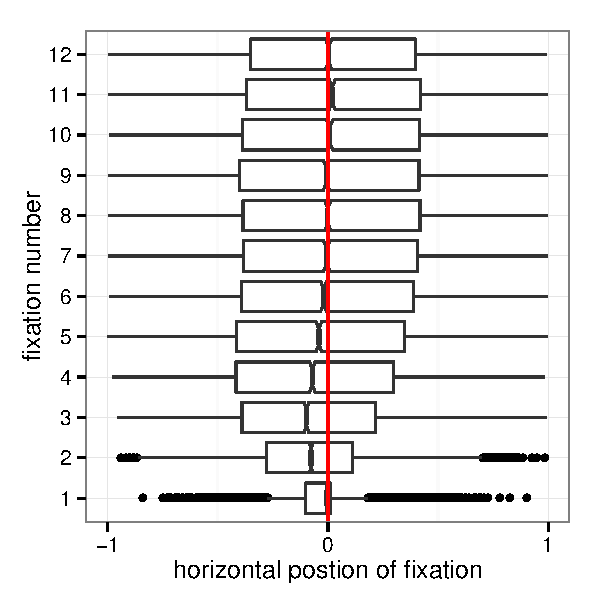
\includegraphics[width=3.8cm]{../scripts/leftVright/graphs/leftrightbias.pdf}}
\subfigure{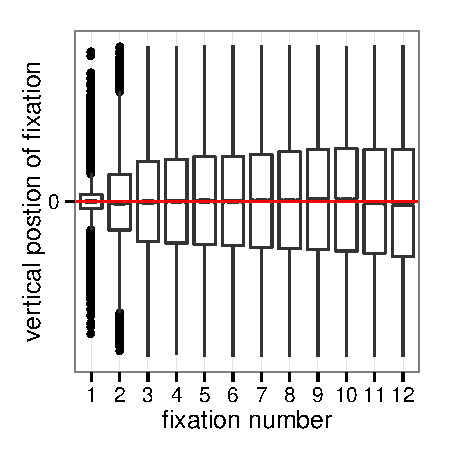
\includegraphics[width=3.8cm]{../scripts/leftVright/graphs/updownbias.pdf}}
\caption{Distribution of horizontal and vertical fixations by fixation number.}
\label{fig:leftrightDist}
\end{figure}

However, it has only a very small effect on explaining the varition over whole datasets: fitting an ANOVA to predict the $x$ coordinates of the fixations given the fixaiton number gives adjusted $R^2=0.004$. If we limit our analysis to the first 5 fixations in each scanpath, this only increases to adjusted $R^2=0.01$. 

Hence we will ignore this effect from now on. By treating everything as symmetrical, we lose very little explanitory power, while restricitng the number of parameters, or increasing the amount of data available (by mirroring fixations). 

\subsection{Saccadic Flow}
\label{ModellingFlow}

Saccadic flow can be thought of as a generalisation of the central bias. Instead of computing the distribution of all saccadic endpoints in a dataset, we look at the distribution of saccade endpoints given the start points. So for a saccade from $(x_0, y_0)$ to $(x_1, y_1)$ we want to model $p(x_1,y_1|x_0, y_0)$ This is illustrated in Figure \ref{fig:empiricalSaccadicFlow}.

\subsubsection{Modelling}


To characterise how the distribution of saccadic endpoints varies with the start point, we used a sliding window approach. All saccades that originated in a $n\times n$ window were taken and used to fit a multivariate Gaussian distribution. This window was then moved over the stimuli in steps of $s=0.01$. Parameter sets estimated from windows containing less than 250 datapoints were removed. Multivariate polynomial regression was then used to fit 4-th order polynomials to each of the parameters. Robust estimation was used (\texttt{rlm} from the texttt{MASS} library) to stop the model fits being overly infleunced by outlier points from the image boundary. We experimented with varying the window size ($n\in\{0.05,0.1, 0.2\}$). However, as this parameter was found to have a negligible result, we only report the results for $n=0.05$.

\subsubsection{Results}

Figure \ref{fig:nParamsOverSpace} shows how the parameters for the multivariate Gaussian distribution vary over horizontal position for a selection of vertical positions. The regression coefficients (given in supplementary materials) allow us to estimate the conditional probability of a saccade to $(x_1, y1)$ given the starting fixation $(x_0, y_0)$.

\begin{figure*}
\centering
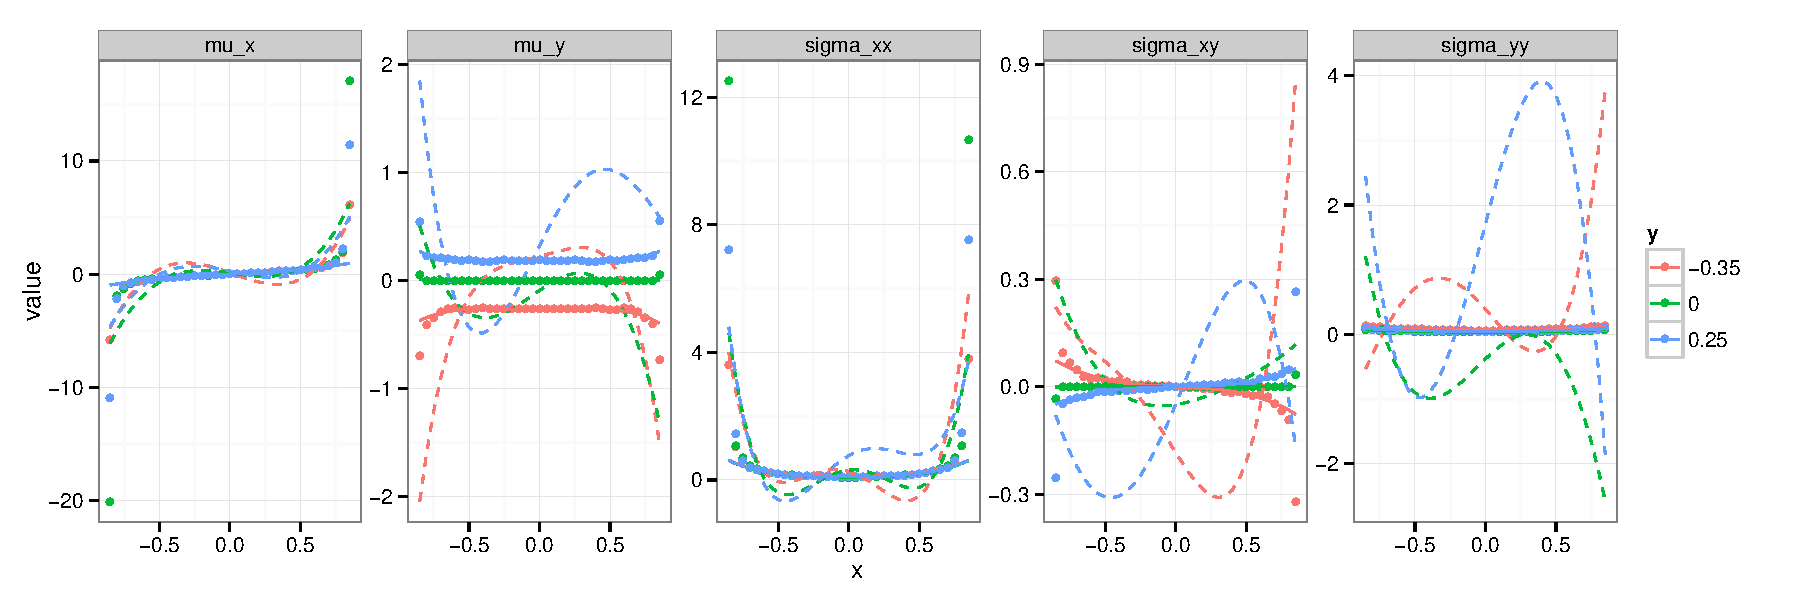
\includegraphics[width=16cm]{../scripts/flow/figs/NparamsChagingOverSpace_ALL_tN}
\caption{How the truncated Gaussian parameters vary with saccadic starting location. Dotted line show polynomial regression fits, solid line shows robust polynomial regression.}
\label{fig:nParamsOverSpace}
\end{figure*}


How well does this model account for the fixations in our datasets? Figure \ref{fig:nFlowDevAll} shows the deviance of the flow model expressed as a proportion of the deviance of the Clarke-Tatler central bias. For reference, we also show the results for re-fitting the central bias to each dataset. From this figure, we can see that the flow-normal model approximately halves the deviance. 

\begin{figure*}
\centering
 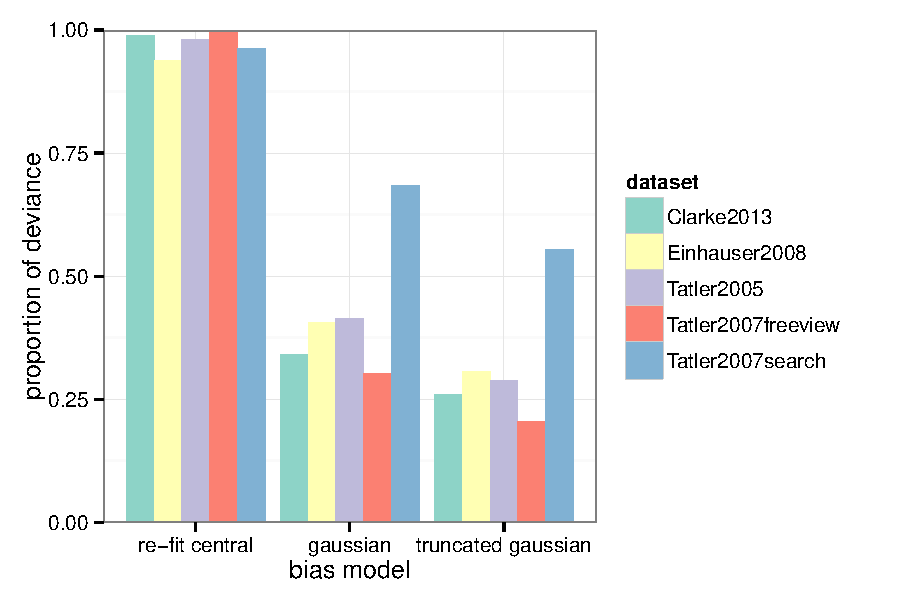
\includegraphics[width=12cm]{../scripts/flow/figs/llh_ALL.pdf}
\caption{Flow:normal log likelihood results. We can see that re-fitting the central-bias to each specific dataset offers little improvement over using the Clarke-Tatler model, while the flow model offers a substantial improvement.}
\label{fig:nFlowDevAll}
\end{figure*}

As the flow:normal model is significantly more complex, requiring nine times as many parameters, it is important to test for robustness. We can test how well our model generalises on testing it on other datasets, for example, \cite{borji2015}. 


\begin{figure*}
\centering
 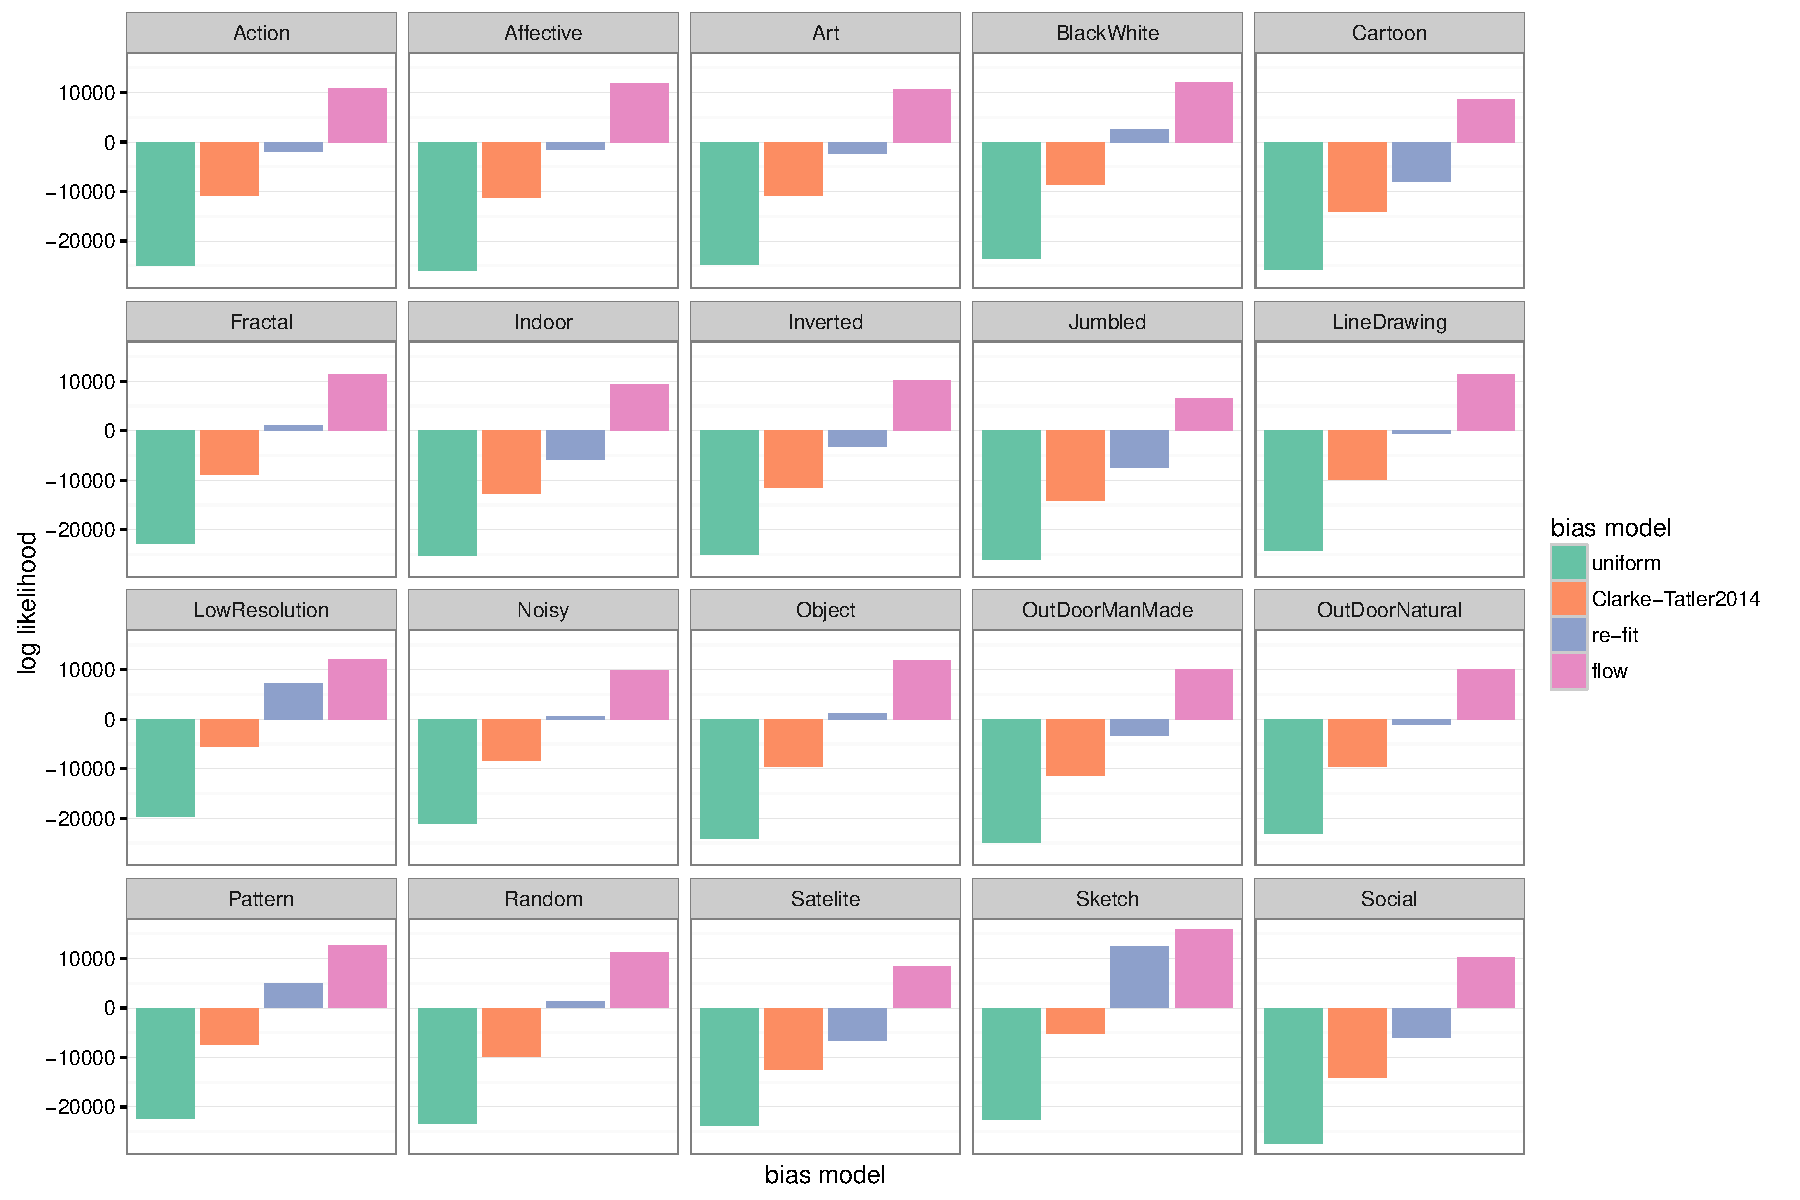
\includegraphics[width=12cm]{../scripts/flow/figs/llh_Borji.pdf}
\caption{Flow:normal deviance results. We can see that re-fitting the central-bias to each specific dataset offers little improvement over using the Clarke-Tatler model, while the flow:normal model decreases the deviance by half.}
\label{fig:nFlowDevBorji}
\end{figure*}

% \begin{figure}
% \centering
%  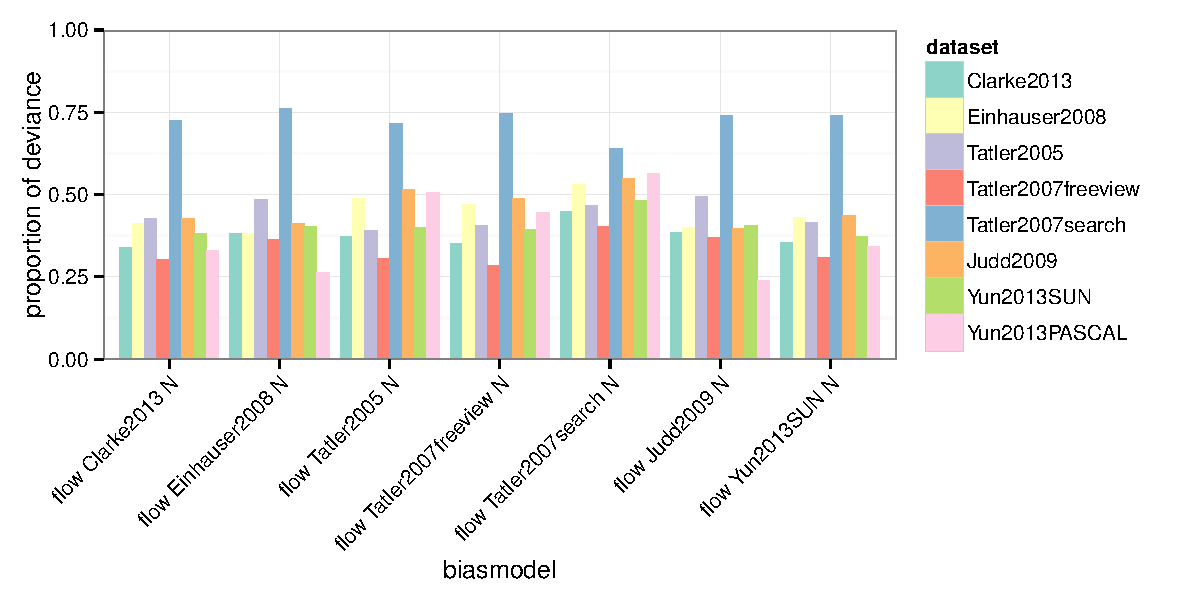
\includegraphics[width=12cm]{../scripts/flow/figs/llh_crossDataset.pdf}
% \caption{Flow:normal deviance results over datasets. In general, we can see that bias models trained on different datasets all explain around the same amount of variance in the datasets.}
% \label{fig:nFlowDevCross}
% \end{figure}

\subsubsection{Discussion}

We put the Flow:normal model forward as a robust prior for image-content independent saccadic behaviour. This model can be thought of as as partner of the Clarke-Tater central bias, and we expect that in some cases, the simpler central bias will be more appropriate, while in others, the more complex flow model is a better choice. We have demonstrated that although this model requires more parameters, it generalises well from one dataset to another and is a far better baseline for modelling a scan-path than the central bias.

There are two main simplifications to our modelling work. First of all, we are using an unbounded distribution (ie, $(x,y)\in \mathbb{R}^2$) to model bounded data. While it is possible to deal with this issue, by either applying a transform $(-1,1)\rightarrow \mathbb{R}$ (such as $z=log(\frac{x'}{1-x'})$, where $x'=\frac{x+1}{2}$), or fitting a truncated multivariate Gaussian, we decided that given the good performance of the model as is, it was not worth adding the additional complexities to our model at this time. 

The second simplification is that we are treating the data as normal. From Figure \ref{fig:empiricalSaccadicFlow} we can see that the data is clearly skewed, particularly in the corners. We will attempt to address these issues in the following section.

\section{Discussion}


\subsection{Scenes and natural viewing behaviour}
That observers organise their viewing behaviour on computer screens around the reference frames provided by the bounds of scenes (see also \cite{Stainer:2013ce}) causes problems for relating findings of eye guidance in scenes to eye guidance in natural behaviour, as the bounds of such reference frames are unclear in the real world. While it has been suggested that we tend to fixate near to the centre of our `straight ahead' head position [FOULSHAM WALKING, CRISTINO AND BADDELEY?], there are no discrete edges as are typical in computer based scene viewing paradigms. If fixation locations are constrained by the bounds of the scene, this highlights the care we must take about the generalisations we make from findings in the lab to the real world (see [kingstonepaper 2010]). 


\section*{Acknowledgements}

%Thanks to Adelchi Azzalini for advice on using the \texttt{sn} package for \texttt{R}. And mention grants. 

\appendix
\section{Dataset Details}

Here are all the details on the datasets used in this paper. (Table \ref{tab:datasets} and \ref{tab:setuptable}).


\begin{table*}
\centering
\small
\begin{tabular}{l|llll}
 						& Observers & Images &  Task & Display duration\\
\hline
\cite{clarke2013}     	& 24   	& 100   & object naming & 5000 ms\\
\cite{yun2013} - SUN    & 8     & 104   & image description & 5000 ms\\
\cite{tatler2005}     	& 14    & 48    & memory 			& variable\\
\cite{einhauser2008} 	& 8		& 93    & object naming 	& 3000 ms \\
\cite{tatler2007} - free & 22   & 120   & free viewing      & 5000 ms\\
\cite{judd2009}         & 15 	& 1003  & free viewing 		& 3000 ms\\
\cite{yun2013} - PASCAL & 3 	& 1000  & free viewing 		& 3000 ms\\
\cite{tatler2007} - search & 30 & 120	& visual search 	& 5000 ms\\
\hline
\cite{clarke2009} 		& 7		& 360	& visual search 	& variable\\
\cite{ehinger2009}     	& 14 	& 912 	& visual search 	& variable\\
\cite{asher2013}    	& 25    & 120   & visual search		& variable\\
\cite{jiang2014}  		& 16 	& 500 	& free viewing  	& 5000 ms \\
\cite{borji2015}  		& 120	& 4000  & free viewing		& 5000 ms\\
\end{tabular}

\caption{Summary of the 13 datasets used throughout this study. The top eight datasets were used to train the model, while the bottom five were only used for evaluation.}
\label{tab:datasets}
\end{table*}

\begin{table*}
\begin{center}
\small
\begin{tabular}{l|llllll}
 & Eye tracker & \vtop{\hbox{\strut Viewing}\hbox{\strut distance}}
 & \vtop{\hbox{\strut Screen}\hbox{\strut size}}
 & \vtop{\hbox{\strut Image}\hbox{\strut size}}
 & \vtop{\hbox{\strut Viewing}\hbox{\strut angle}}
 & \vtop{\hbox{\strut Chin /}\hbox{\strut head rest}}\\
\hline
\cite{tatler2005} 			& EyeLink I 	& 60 cm 	& 17" 	& $800 \times 600$ 	& $30 \times 22^{\circ}$ 	& no\\
\cite{tatler2007} - free 	& EyeLink II 	& 60 cm 	& 21" 	& $1600 \times 1200 $	& $40 \times 30^{\circ}$ 	& no \\
\cite{tatler2007} - search 	& EyeLink II 	& 60 cm 	& 21" 	& $1600 \times 1200$ 	& $40 \times 30^{\circ}$ 	& no\\
\cite{einhauser2008} 		& EyeLink 1000 	& 80 cm 	& 20" 	& $1024 \times 768$ 	& $29 \times 22^{\circ}$ 	& yes\\
\cite{judd2009} 			& ? 			& 2 feet 	& 19" 	& $1024 \times 768*$ 	& ? 				& yes\\
\cite{clarke2013} 			& EyeLink II 	& 50 cm 	& 21" 	& $800 \times 600$ 	& $31 \times 25^{\circ}$ 	& no\\
\cite{yun2013} - PASCAL 	& EyeLink 1000	& ? 		& ? 	& ? 			& ? 				& ?\\
\cite{yun2013} - SUN 		& EyeLink 1000 	& ? 		& ? 	& ? 			& ? 				& ?\\
\hline
\cite{clarke2009} 			& Tobii x50 	&87 cm			& 20"		& $1024\times 1024$	&	$16.7\times16.7^{\circ}$ & yes \\
\cite{ehinger2009} 			& ISCAN RK-464 	& 75 cm 	& 21" 	& $800 \times 600$ 	& $23.5 \times 17.7^{\circ}$& yes\\
\cite{asher2013} 			& EyeLink 1000 	& 55 cm 	& ? 	& $1024 \times 1280$& $37.6 \times 30.5^{\circ}$& yes\\
\cite{jiang2014}  			& Eyelink 1000 	& 57 cm		& 22"	& $1024 \times 768$ & $38.8 \times 29.1^{\circ}$& ?\\
\cite{borji2015} 			& Eyelink 1000	& 106 cm	& 42" 	& $1920\times1080 $	&$45.5\times31^{\circ}$& yes \\
\end{tabular}
\end{center}

\caption{Details of the experimental setups in each of the 10 datasets analysed in the present study. We provide only information reported in the original articles. Question marks indicate information not reported in the original article. *For the Judd et al dataset images varied in pixel dimensions but the majority were at 1024 x 768.}
\label{tab:setuptable}
\end{table*}

\bibliographystyle{plainnat}
\small
\bibliography{literature}
\end{document}